\documentclass[12pt,a4paper]{report}

\usepackage{amsmath}
\usepackage{amsfonts}
\usepackage{amssymb}

%\usepackage{tocloft}

%glossar
%\usepackage[xindy]{glossaries}

% Bibliography Quellen.
% Immer nur eine verwenden
%\usepackage{natbib} % Zitate mit Namen + Jahr
\usepackage{cite} % Zitate mit Nummern

% Eigene Style-Datei mit weiteres Includes
\usepackage{projekt}

\usepackage{algorithm2e}
\newtheorem{defi}{Definition}[chapter]
\usepackage{tabularx}

% Pakete f�r Links
\usepackage{hyperref}
\usepackage{url}
\usepackage{subcaption}
\usepackage{enumerate}
\usepackage{graphicx}  % remove 'demo' option for your real document
\usepackage[toc]{appendix}


\usepackage{glossaries}
\makeglossaries


\author{Dennis Sebastian Rieber}
\title{Characterization Of GPU Communication}
\setTopic{A Scientific Exploration}
\setFackultaet{Department of Physics and Astronomy}
\setBetrieb{University of Heidelberg}
\setInstitute{ZITI, Computer Engineering Group}
\setSupervisor{JProf. Dr. Holger Fr�ning}
\setStudiengang{Computer Engineering}

\begin{document}
% Set Font (If we don't want times)
%\changefont{phv}{m}{n} % (SansSerif) Helvetica
%\changefont{ppl}{m}{n} % Palantino
%\changefont{pnc}{m}{n} % New Century Schoolbook

% preface with roman numbers
\maketitle
%\newpage % Newpage required for correct pagination
\begin{abstract}
% Moti
GPU hardware and software continues to scale and understanding applications is crucial for performance
optimizations.
% Problem statement
To the knowledge the author, there is no work concerned with the intra-applications communication in GPUs and
no instrumentation framework capable of dynamic tracing at GPU runtime.
%Approach 

This work uses compiler extensions to instrument GPU applications for tracing. The instrumentation adds tracing for all load and store instructions targeting global memory in a GPU. Data is dynamically transferred between from the device to host at run time, through a producer-consumer controlled buffer. 
%results

Using the generated traces, communication across BSP supersteps is analysed. The analysis shows messages between supersteps are dominated transfer few sizes. The number of communication partners and memory strides
of communication depend on the application and its regularity.
%conclusion
\\\\
Das ist der Deutsche Abstract
\end{abstract}

% Roman counting for ToC
\setcounter{page}{1}
\pagenumbering{Roman}
\setcounter{page}{1}
\tableofcontents
\newpage % Newpage required for correct pagination

% 1.5 linespacinfg
%\singlespacing
\onehalfspacing

\clubpenalty = 10000 % schliesst Schusterjungen aus 
\widowpenalty = 10000 \displaywidowpenalty = 10000% schliesst Hurenkinder aus

% Equation listing
\newcommand{\listequationsname}{Gleichungsverzeichnis}
%\newlistof{myequations}{equ}{\listequationsname}
\newcommand{\myequations}[1]{%
\addcontentsline{equ}{myequations}{\protect\numberline{\theequation}#1}\par}

%\lstlistoflistings\newpage
\listoffigures\newpage
\listoftables
	%\include{praeamble}
	% Document with regular arabic pagination
	\pagenumbering{arabic}
	\setcounter{page}{1}
	\chapter{Motivation}
\begin{itemize}
	\item GPUs are not CPUs. Different design philosophy leads to different application optimizations
	\item GPU's concurrent hardware continues to scale
	\item therefore optimizations of data movements, consistency etc. are required to harness compute power of new hardware generations
	\item Complex Applications have non-trivial communication patterns in data parallel kernels, which are not researched yet.
	\item This work is aimed to generate understanding of communication patterns to help build and optimize Tools (Mekong etc.) and Applications
	\item Generate Traces with compiler instrumentation because
	\item ...Process simulators to slow for real applications and only support outdated Architectures (GPUSim only supports up to Fermi)
	\item ...analytical modelling usually lack the accuracy to capture exact patterns in complex communication since they are based on simplifications
	
\end{itemize}
\section{Goal}
The Goal of this Thesis is to develop instrumentation for dynamic global memory tracing in GPU applications. The instrumentation will happen at compile time using custom plugins for Clang and LLVM to transform the source code of the
original application. With this setup, traces can be generated with any application that provides source code and
across different generations of NVidia hardware. A loss in performance resulting from the traces will be tolerated.

The generated traces will be used to analyse how CTAs and kernels communicate during the execution of an application. 
The communication will be analysed on a qualitative level by classifying how the data is exchanged and on a quantitative level with metrics like volume, frequency and density to describe kernel and CTA interactions.

\section{Outline}
	\paragraph{Chapter 2} presents technological background information. It will introduce BSP, GPUs, LLVM, SSA and the compiler techniques used to transform the code of the original application.
	\paragraph{Chapter 3} discusses work related to this Thesis. It will explore work in the field of code instrumentation and GPU performance analysis.
	\paragraph{Chapter 4} defines what communication in the context of this work and explores the analysis space.
	\paragraph{Chapter 5} presents how the tracing is realized including the compile stack, AST manipulation and deeper code analysis in LLVM's intermidiate representation (IR).
	\paragraph{Chapter 6} presents the set of applications that will be analysed, the different metrics are explained in detail and the results of the analysis are discussed in length.
	\paragraph{Chapter 7} concludes and summarizes the results of this Thesis and discusses possible future directions this project could take.

	\chapter{Background}
\section{Bulk Synchronous Parallel} \label{sec:bsp}
Bulk Synchronous Parallel (BSP) is a bridging model introduced by L.G. Valiant in \cite{Valiant:1990:BMP:79173.79181}. A bridging model describes a conceptual understanding of
hardware for the purpose software development. The most basic of these models is the von Neumann architecture, which is still used as the basic understanding of sequential hardware in modern CPUs. In the wake of parallel computing, BSP was proposed to fulfil the same roll
for the understanding of parallel hardware. The model does not specify how any of the elements should be realised in hardware or software, since it's purpose is to provide a common ground for hardware and software developers. 
BSP fundamental principal is the separation of computation and communication. A computer modelled after BSP requires
\begin{enumerate}
	\item a set of components or execution units, performing the computational work of the algorithm.
	\item a router to convey information between the components.
	\item a facility to synchronize some or all of the components in steady intervals.
\end{enumerate}
Each component performs local computations and then shares its results with
the other components via the rounter. The synchronization guarantees that all components completed computation and communication. The sequence of computation, communication and synchronization is called a superstep. One or more supersteps are used to implement an algorithm.
The model allows excluding components from synchronization, if the algorithm allows or requires it.

Although all computations are supposed to be local, BSP allows concurrent read and concurrent write access to a shared memory between the
components. But this is only allowed, if the underlying memory system guarantees coherent and consistent resolution of access conflicts.

\section{General Purpose GPU Compuing}
GPGPU computing utilizes GPUs for computations other that graphics. With CUDA, NVidia offers a C-based, proprietary language to write application for NVidia GPUs. GPUs are so called "many-core" processors, with thousands of compute units (CUDA cores). CUDA cores are clustered in Streaming Multiprocessors(SM), executing 32 threads concurrently. Code executed on a GPU is capsuled in a kernel. Figure \ref{gpu-hier} is an overview of the features detailed in the next sections. Nvidia also offers an assembler-like language called PTX, that is not architecture generation specific. \cite[4.1-4.2	]{cuda-man}

\subsection{Execution Model}
Threads is CUDA are hierarchically organized. Groups of up to 1024 threads are organized in a 3D block, called "Collaborative Thread Array" (CTA). The execution of one compute kernel consists of many CTAs, organized in a 3D grid. During a kernel execution, the CTAs are  scheduled to a SM in a non-deterministic fashion, based on available resources. Once a CTA is scheduled, it can not be pre-empted and executes until it is finished.  \cite[2.1 - 2.2]{cuda-man}

The threads inside a CTA are organized in groups of 32, called warp. All threads in a warp execute the same instruction stream. If the one or more threads in a warp have a branch in the Control-Flow-Graph (CFG), all threads in the warp
execute the branch, but only the ones supposed to work create side-effects. The shared instruction stream continues if all threads finished a branch. \cite[4.1]{cuda-man}

A kernel usually consists of more CTAs than a GPU can execute concurrently. Non-deterministic scheduling on the GPU  prevents predictions on the CTA execution order, making CTA interaction
in a kernel a deadlock hazard. Therefore interaction of threads belonging to different CTAs are not allowed. The execution model allows threads inside the same CTA to interact using Shared Memory, which is located in the SM and private for each CTA. \cite[5]{cuda-man}

Kernels are executed in the order in which the kernel calls are issued by the application. CUDA streams allow concurrent  execution of multiple kernels and data movement, given the resources are available on the GPU. \cite[5]{cuda-man}

\subsection{Memory Model}
GPUs have a hierarchical memory model, with different address spaces. Table \ref{GPUMemTable} lists all available memories and their properties. For this work we will focus on global memory, as it is the only 
memory allowing modification by a kernel, which persist beyond the kernel completion boundary.
Host-Mapped memory falls in the same category as global, and for our purposes is treated as global memory. 
Global address space is a shared memory for all kernels running a GPU.

It is important to note, that CUDA only guarantees a consistent state of global memory, after the kernel completion 
boundary. There are no guarantees on global memory consistency during the execution of a kernel, which is another reason
CTA interaction at kernel run-time is not intended. \cite[B5-B7]{cuda-man}
\begin{figure}[t]
	\centering
	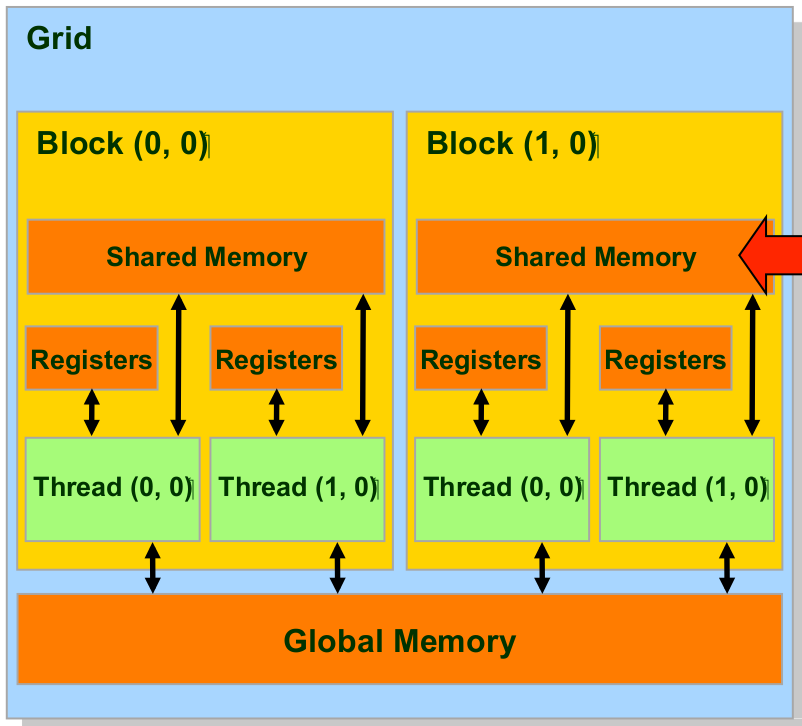
\includegraphics[width=0.6\textwidth]{gpu-arch}
	\caption{GPU thread and memory hierarchy. Image from \cite{}}
	\label{gpu-hier}
\end{figure}
\begin{table}
	\centering
	\begin{tabular}{|l|c|c|c|c|c|c|}
		\hline 
		\textbf{Memory} & \textbf{Scope} & \textbf{Access} & \textbf{Bandwidth} & \textbf{Latency} & \textbf{Capacity} & \textbf{Location} \\ 
		\hline
		\hline
		Register  & Thread & RAM & high & low & 32bit & SM \\ 
%		\hline 
		Shared  & CTA & RAM & high & low & < 48k & SM \\ 
%		\hline 
		Global  & Kernel & RAM & high & high & < 20GB & device \\ 
%		\hline 
		Texture/Constant & Kernel & ROM & high & high & < 20GB & device \\ 
%		\hline 
		Host-Mapped  & Kernel+CPU & RAM & low & high & > 20GB & host \\ 
		\hline 
	\end{tabular} 
	\caption{GPU Memory\cite[2.3]{cuda-man}}
	\label{GPUMemTable}
\end{table}
\section{LLVM}
LLVM is a compiler project providing tools for full-stack compiler development. While originally written for C/C++, nowadays front-ends for many languages are provided and back-ends for many different architectures are available. The C/C++ compiler using the LLVM tool-chain is called Clang. Since 2015 Clang and the LLVM
tool-chain support CUDA code and can produce PTX files for GPU execution \cite{gpucc}.
LLVM uses an intermediate representation (IR) for code analysis and optimization 
(more on this in \ref{llvmir}). Code compiled with Clang is translated into IR and then further processed. \cite{Lattner:2004:LCF:977395.977673}

For this work, we will distinguish the tool-chain into three major components:
\begin{itemize}
	\item The \textbf{front-end} takes care of pre-processing, lexical, and syntactical analysis of the original code. Clang uses an Abstract Syntax Tree (AST) to represent the original code. This AST is accessible via an API and additional plug-ins can be added to the tool-chain. After the lexical and syntactical analysis are complete, the code is translated into IR. 
	\item The \textbf{optimizer} uses the IR to analyse and then transform the code. The IR is accessible with an API and allows the introduction of additional modules for analysis or transformation. These modules are called a "pass" (details in section \ref{llvmpass}).
	\item The \textbf{back-end} includes the linker and back-end architecture depended code generation. This part of the
	toolchain is not relevant for this work and is only mentioned for completeness.
\end{itemize}
This overview gives an sufficient understanding of the LLVM stack for this work and in the following sections
the concepts of IR and passes are explored in more depth.

\subsection{LLVM IR Program Representation} \label{llvmir}
LLVM's IR is a typed RISC instructions set with a load/store memory architecture. The IR is architecture agnostic and provides an infinite set of virtual, typed registers. The available primitive language-independent types are: (un)signed integer (8-64 bit), single and double precision floating point, and Boolean. Derived from these primitive types are the aggregate types pointers, arrays, structures, and functions. In LLVM it is possible to transform form any type into an arbitary other type, using the \verb|cast| instruction. \cite{Lattner:2004:LCF:977395.977673}

Any kind of pointer arithmetic and access to aggregate types is performed by the \verb|getelementptr| (\verb|gep|) instruction, which preserves type information, is machine and language independent, and returns a pointer. Using \verb|gep| allows the IR to keep load/store instructions clean and only use the direct address to access element.
\cite{Lattner:2004:LCF:977395.977673}

One important part of LLVM's code transformations are canonicalization and lowering, which happenin the front-end. One example of lowering is the \verb|gep| instruction, that brings any kind of language intrinsic for address access into the same form. Canonicalization happens for logical constructs in the program's CFG. For example, any loop in a program is brought into the same canonical form before any analysis on the loop is performed.
The reason for this is the simplification and optimization of the passes analysing and transforming the program. 
\cite{llvm-passes}
\subsection{Static Single Assignement}
LLVM's IR is represented in Static Single Assignement (SSA) form. Informally, it can be defined as
"A program is defined to be in SSA form if each variable is a target of exactly one assignment
statement in the program text" \cite[p. 6]{Rastello:2016:SCD:3002539}.
\begin{figure}[t]
	\begin{minipage}{0.43\textwidth}	
\begin{lstlisting}[style=c]
a = 5
b = a + 1
a = 2
c = a + 1
\end{lstlisting}
	\end{minipage}\hfill
	\begin{minipage}{0.5\textwidth}
\begin{lstlisting}[style=c]
a1 = 5
b1 = a1 + 1
a2 = 2
c1 = a2 + 1
\end{lstlisting}
	\end{minipage}\hfill
	\caption[non-SSA vs. SSA code]{The left hand side is non-SSA program text, on the right hand side the corresponding SSA representation. It is customary to use a counting index for successively defined variables in SSA. Variable a's value is changed in line three. Therefore, a new definition is used in the SSA form}
	\label{simpleSSA}
\end{figure}
\subsubsection{$\phi$ Functions}
A simple example of a program and for the corresponding SSA form  is displayed in figure \ref{simpleSSA}.
This example has no branches and would result in a strictly sequential CFG.
Figure \ref{simple-cfg} shows how a branching program creates divergence in the CFG. This creates additional basic blocks,
which then merge back together at the end of the branch. The program used in \ref{simple-cfg} is not in SSA form, as the variable \verb|b| is defined at two different places in the program text. One of the most integral concepts of SSA is used to resolve situations like this.
The $\phi$-function (sometimes called $\phi$-node), is a "pseudo assignment function"\cite{ssabook} which resolves multiple incoming values
at the location a CFG merges back together by defining a new variable that is used in the later program flow.
\cite{Rastello:2016:SCD:3002539}

The $\phi$-function has $n$ parameters for the $n$ incoming edges to the basic block. For the definition of the new variable, it selects
the value belonging to edge actually coming in at runtime. It is important to keep in mind that $\phi$-node are a helper, that is not
actually present in the final program. After analysis and transformation are finished by the optimizer, the SSA form is de-constructed
by the back-end. Now, as values are mapped to registers and memory locations that can be overwritten, the $\phi$-nodes and SSA form are no longer necessary.
\cite{Rastello:2016:SCD:3002539}

\begin{figure}[t]
	\begin{minipage}{0.4\textwidth}
		\begin{lstlisting}[style=c]
if (a = 5)
	b = 3
else
	b = 5
print(b)
		\end{lstlisting}
	\end{minipage}\hfill
	\begin{minipage} {0.45\textwidth}
			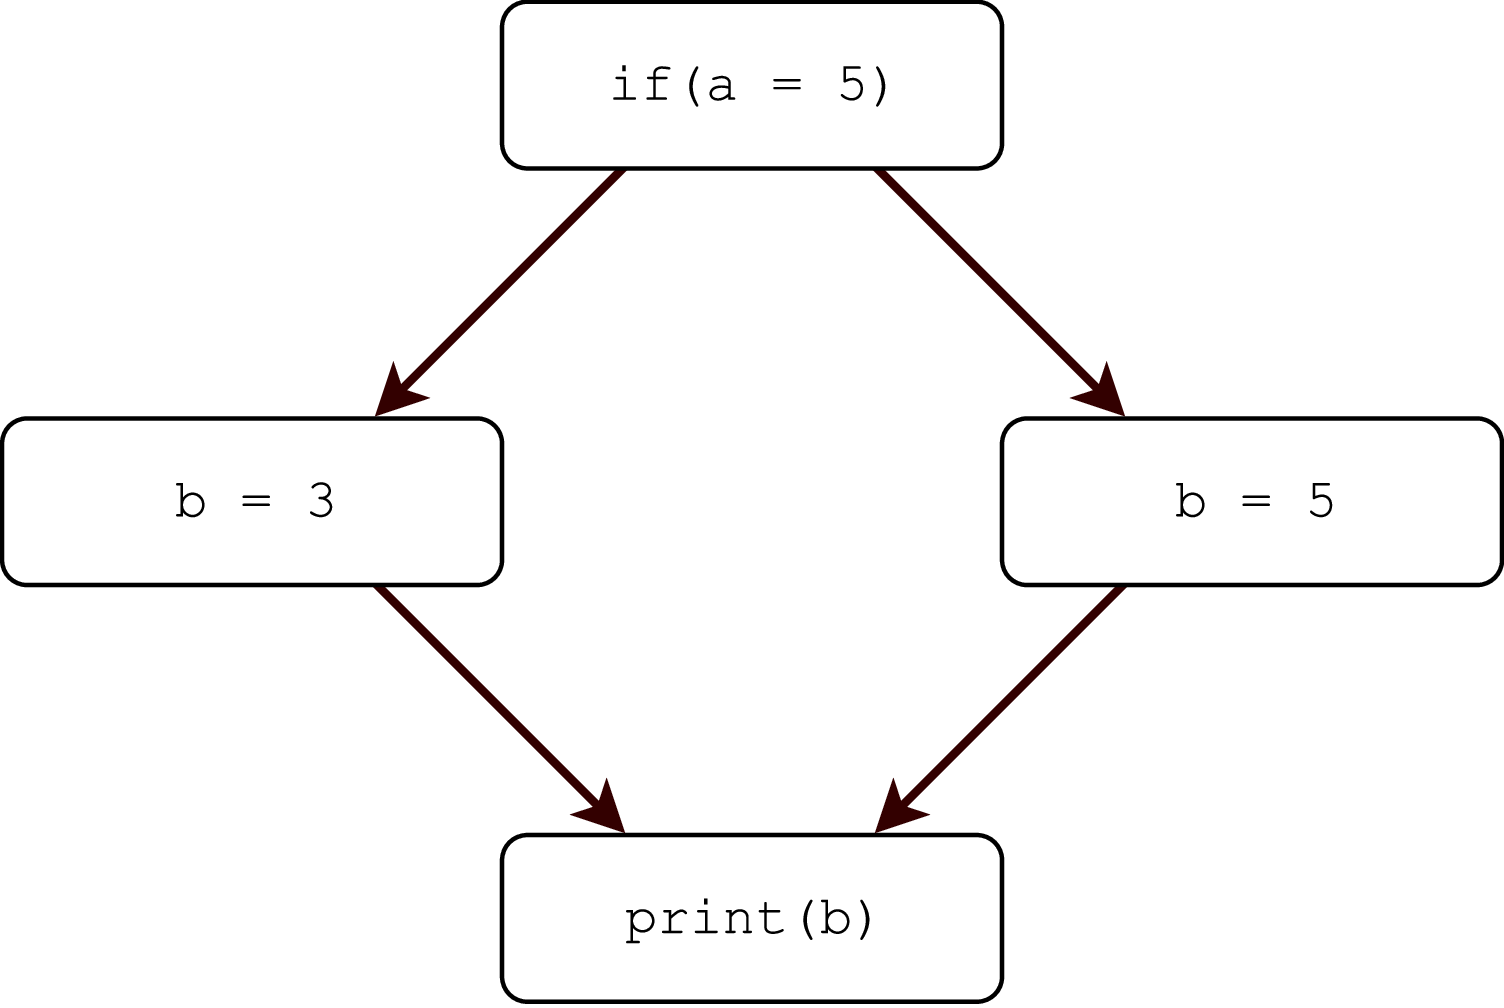
\includegraphics[width=\textwidth]{basic-cfg}
	\end{minipage}
\caption{Branching program and resulting CFG. Not in SSA form.}
\label{simple-cfg}
\end{figure}
\begin{figure}[t]
	\begin{minipage}{0.4\textwidth}
		\begin{lstlisting}[style=c]
if (a1 = 5)
	b1 = 3
else
	b2 = 5
b3 = phi(b1,b2)
print(b3)
		\end{lstlisting}
	\end{minipage}\hfill
	\begin{minipage} {0.45\textwidth}
		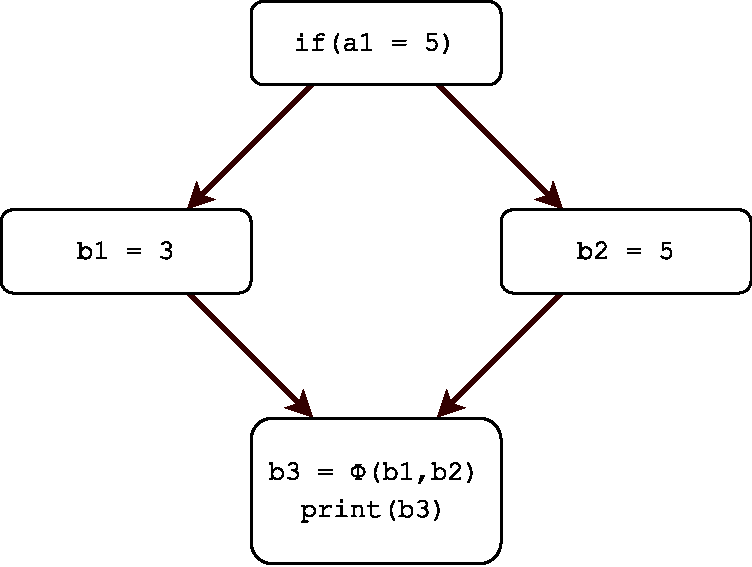
\includegraphics[width=\textwidth]{phi-node-simple}
	\end{minipage}
	\caption{Branching program and resulting CFG. Now in SSA form, with $\phi$-function resolving merging CFG paths}
	\label{simple-phi}
\end{figure}
\subsubsection{Def-Use and Use-Def Chains}
An important data structure in compiler analysis are def-use and use-def chains. The former is list of every use a definition has. Use-def chains point backwards to all definitions of variable, from the perspective of a use.  
\cite{Rastello:2016:SCD:3002539}

Due to the single definition variables of SSA, use-def chains are a single name, or element. Def-use chains can be build easily because they can be constructed through the single element use-def chains. We look at each use in the program and add the user to the definition's def-use list. Def-Use connections enable fast forward travelling through a CFG, because one is not bothered with code that is not part of the def-use chain. Figure \ref{def-use} shows an example of def-use connections for the variable \verb|a1|. The use-def connections would be the inversion of the dotted arrows. \cite{Rastello:2016:SCD:3002539}
\begin{figure}[t]
	\centering
	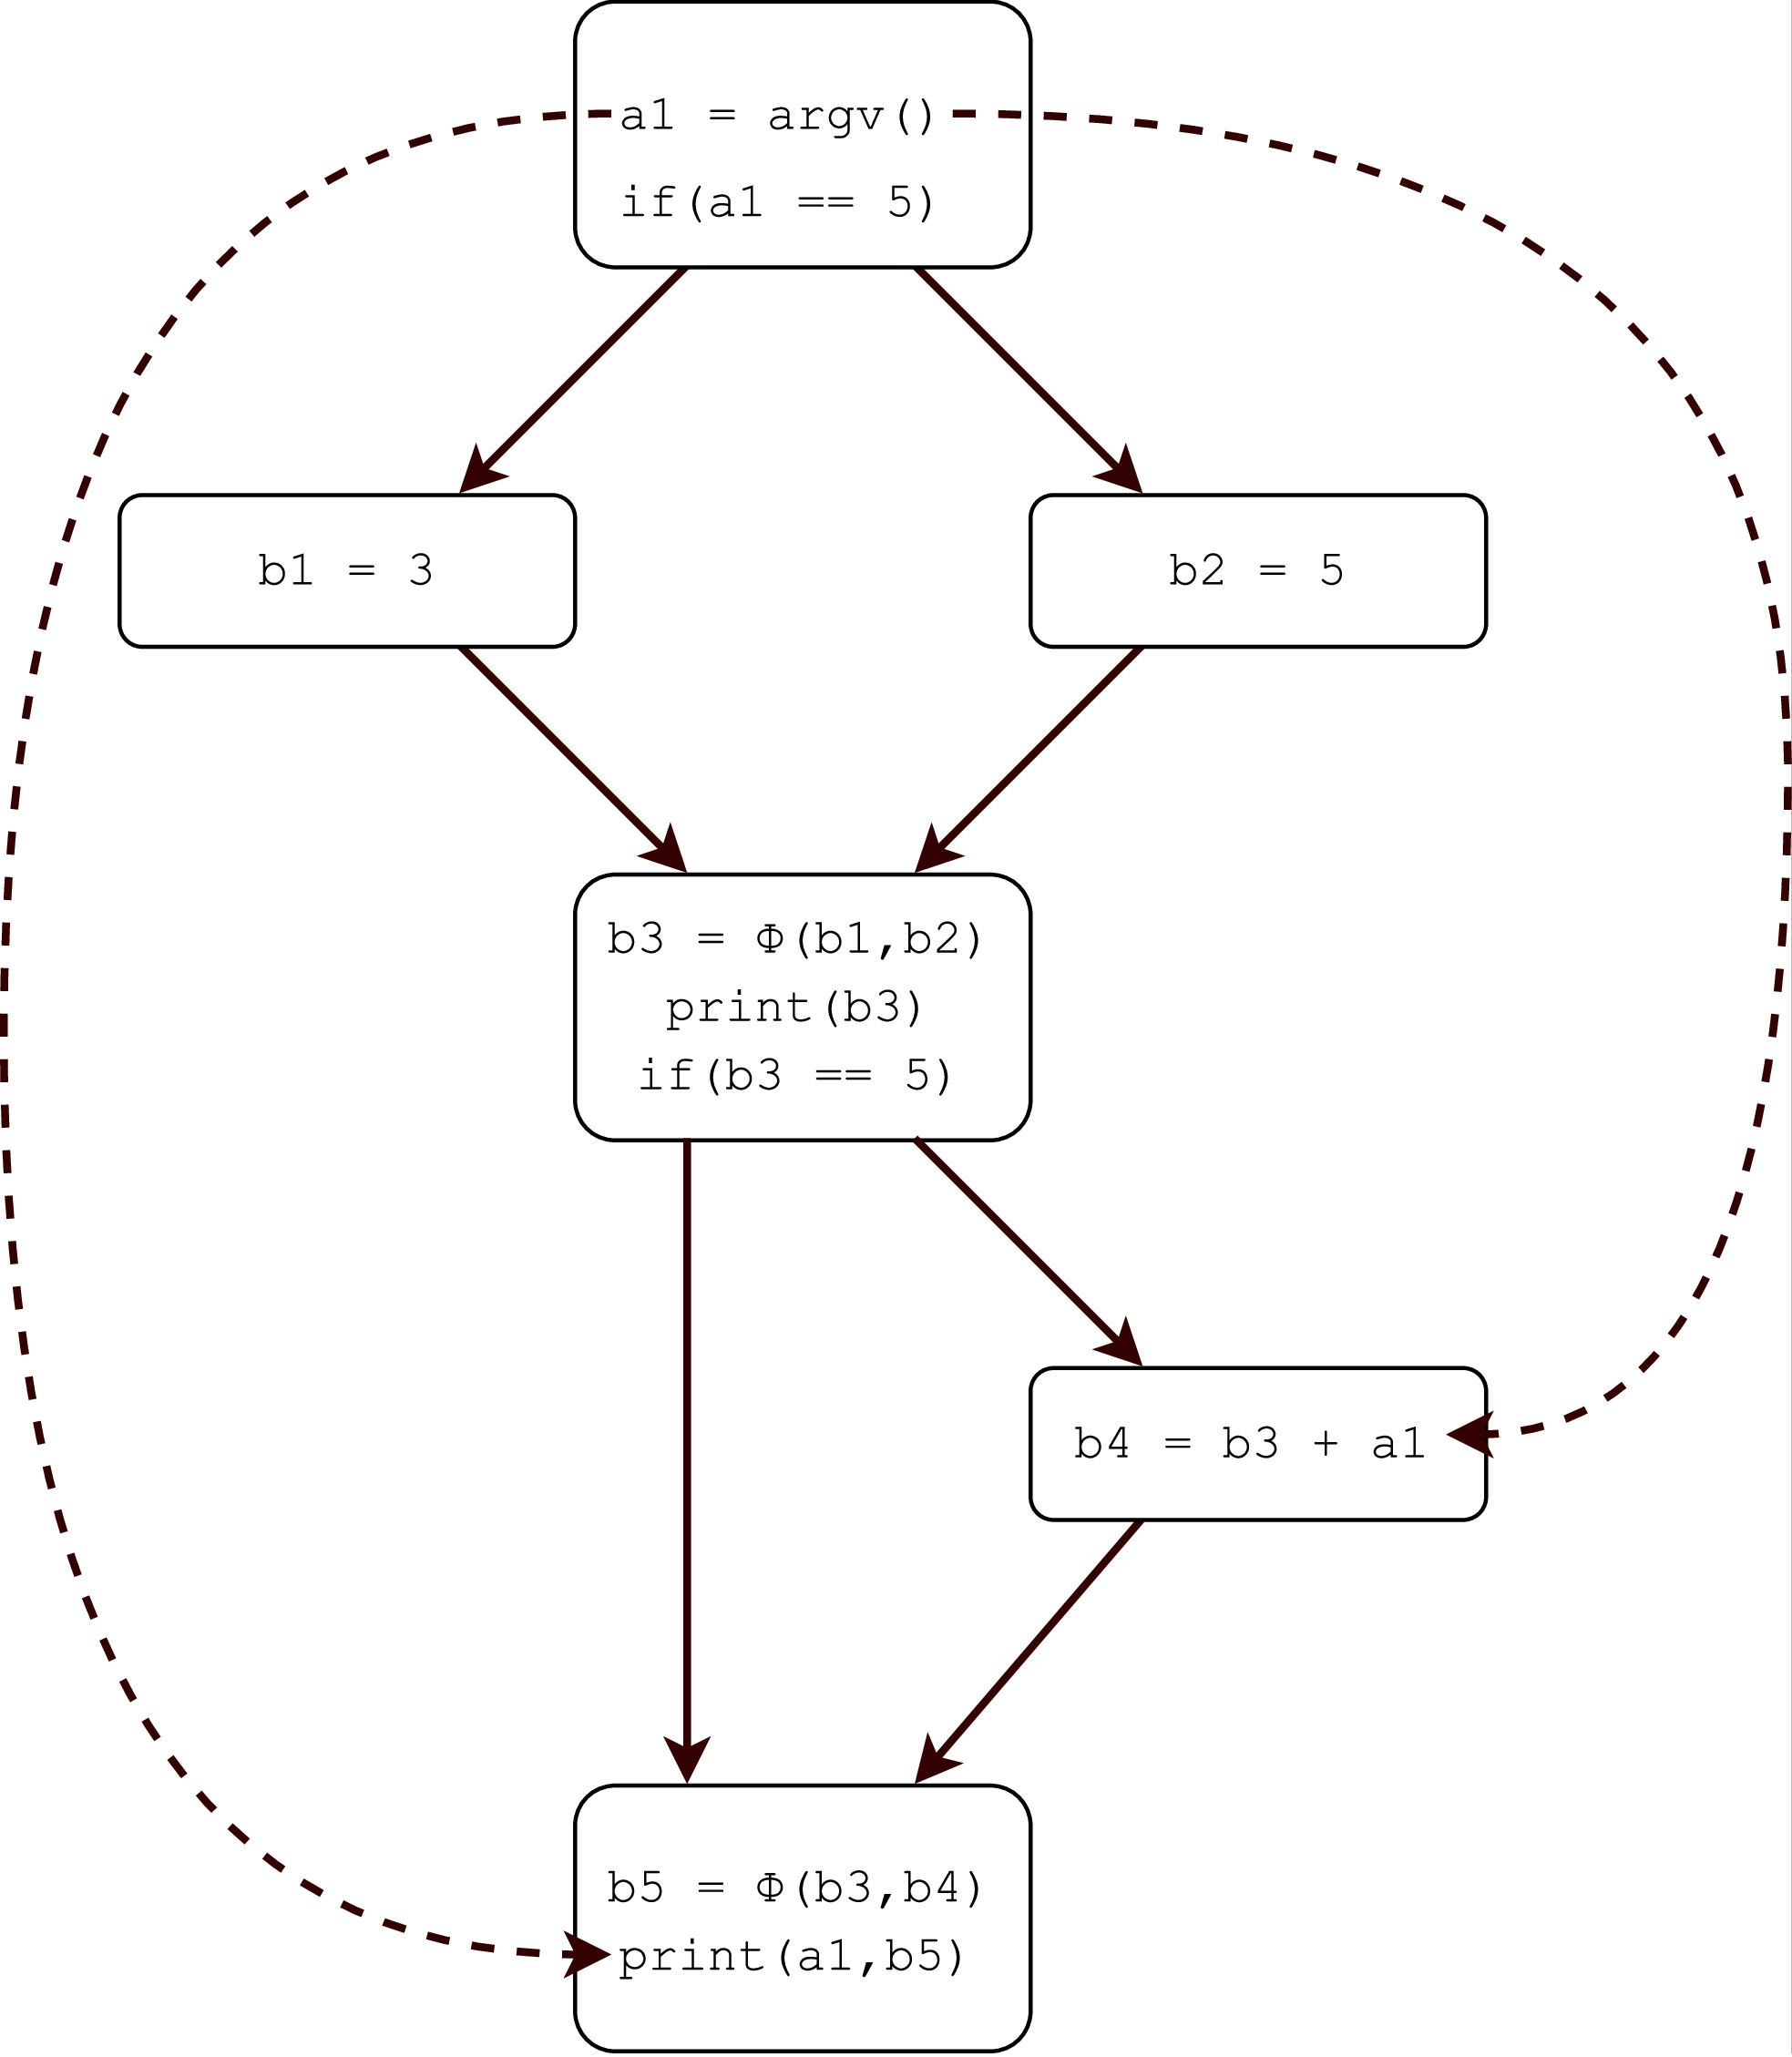
\includegraphics[width=0.6\textwidth]{def-use}
	\caption{Def-Use connections of variable a1, displayed as dotted lines.}
	\label{def-use}
\end{figure}

\subsection{LLVM Pass}\label{llvmpass}
A pass in LLVM is piece of software responsible for an analysis or transformation of IR. Passes are distinguished into said categories. An analysis pass creates or computer some information on the piece of IR it is running on, which later can be used by other passes. It doesn't modify the IR. As one pass may depend on the result of another analysis, passes are scheduled accordingly by the pass manager. A transformation pass alters the IR in place and does not produce any results. A transformation might trigger the re-run of an analysis as changes to the IR might invalidate the original results. Opposed to an analysis, transformations are not allowed to rely on results of other transformations. \cite{llvm-passes}

\subsubsection{Scopes}
A pass can run various scopes of IR. The pass can not access IR outside this scope and in the same pass, information can not be conveyed from one context to the next. For example: If a pass analyses functions, each function in the IR is analysed individually, with no knowledge about other functions. \cite{llvm-scopes}
\begin{itemize}
	\item \textbf{Module} scope contains the whole compilation unit with all it's functions and definitions. It is largest scope available.
	\item \textbf{Function} scope looks at every function individually. As the pass is limited to a function definition, it has no calling-context information. 
	\item \textbf{Loop} scope only provides access to the loop head and body, including loops nested into the loop.
	\item \textbf{BasicBlock} can only access a single basic-block. No CFG manipulation possible.
\end{itemize}

\section{Compiler Techniques}
This section will briefly introduce terminology for two types of analysis and transformation a compiler can perform, which are relevant
for this work.
\subsection{Data Flow Analysis}
Data flow Analysis is a broad field, with some shared terminology that is described here. Generally, such an analysis traverses the code,
search for specific facts and optimizing the code according to the analysis results. Examples are constant propagation or zero value propagation. It is also closely related to pointer analysis, in terms of terminology and overall structure.
\begin{itemize}
	\item \textbf{Property Space} is a set of analysis facts. Represented as partially ordered sets with anti-symmetric, transitive and reflexive relation.\cite{Rastello:2016:SCD:3002539}
	\item A \textbf{Transfer function} classifies each visited analysis object, and determines to which set of the property space an object belongs to. To avoid loops, the transfer function needs to be monotonic. \cite{Rastello:2016:SCD:3002539}
	\item \textbf{Program Representation} is how the program is represented during the analysis. Usually, it is the CFG, but more sparse representation like def-use connections can be used as well. \cite{Rastello:2016:SCD:3002539}
	\item \textbf{Context Sensitive} describes the attribute, that the analysis of a function is sensitive to the context the function is called in. For example, the function
	takes the functions arguments into regard. \cite{Emami:1994:CIP:178243.178264}
	\item \textbf{Flow Sensitivity} defines that the sequence of instructions is of importance for the analysis. \cite{Hardekopf:2009:SFP:1480881.1480911}
\end{itemize}

\subsection{Function Specialization}
Specialization (sometime procedure cloning) create distinct versions of a functions for a specific purpose at compile time. The technique was first introduced in \cite{Cooper:1993:MPC:2245763.2246020}. It resembles templates in C++, creating a function for every template used argument. A specialized function relies on information gathered during the analysis create a specialized version. An example for this are functions with differently unrolled loops, depending on the calling context of the function.

It differs from inlining, because it doesn't interfere with the original code structure. The difference to traditional data-flow analysis based optimizations is that it's possible to create multiple specialized versions for multiple data-flow facts, that vary depending on the calling context.   
	\chapter{Related Work}
\section{GPU Application Characterization}
Since GPGPU computing exists, there are publications characterizing GPU application. Generally, the analysis
aspects can be separated into high-level, low-level . The former treats an application as a black-box
and measures behaviour of the complete application. Latter inspects hardware level behaviour without
beeing concerned, which part of the program is executed. Most research papers report how changes in software or hardware influence certain aspects of low-level or high-level analysis.

High-level research often reports speed-up resulting from a change in hardware or software. Abe et al. \cite{6877247} report on power efficiency and performance. 
It is also concerned with configuration, such as launch configurations and number of kernels (\cite{6983039}, \cite{Kerr:2009:CAP:1678998.1680778}). Wang et al. \cite{6983039} report on how dynamic programming affects kernel count and launch configurations of irregular workloads. Subsequently the report how this affects low-level metrics like memory access and control flow.

Low-level can be devided into memory and exection.
Research concerned with GPU memory behaviour report L2 cache hits/efficiency (\cite{microarch}), global memory load/store counters (\cite{microarch}, \cite{6983039}) or use these numbers together with instruction replay and coalescing to create metrics like memory intensity (\cite{Kerr:2009:CAP:1678998.1680778}) or regularity (\cite{Burtscher:2012:QSI:2473499.2474126}).  Execution research is concerned with control-flow, instruction counts, and occupancy (\cite{microarch}, \cite{Kerr:2009:CAP:1678998.1680778}).

To the best  knowledge of the author, there are no publication researching intra-application interactions.
%\begin{itemize}
%	\item Usually see Application not as a set of different kernels and ignore kernel "interactions"...
%	\item ... or go down to instruction/warp 
%	\item ... or look at architectural impacts on applications
%	\item A Characterization and Analysis of PTX Kernels
%	Andrew Kerr, Gregory Diamos, and Sudhakar Yalamanchili: Broad overview on many applications. Simulated PTX execution, Memory Intesity, branch divergence etc.
%	\item Most other Papers analyse on similar levels, focussing on different Application or Architecture Aspects
%\end{itemize}
\section{GPU Code Instrumentation}
Instrumenting existing application with addition code for memory tracing is essential for this work.
A framework for code instrumentation is presented in "Lynx: A Dynamic Instrumentation System for Data-Parallel Applications on GPGPU Architectures" \cite{Farooqui:2012:LDI:2310660.2310989} by Farooqui et al. Lynx is a framework including a C-to-PTX JIT, that extends CUDA code on PTX instruction level and a runtime, displayed in \ref{lynx-rt}. The user writes instrumentation specification in a C-style language. The specification is translated to PTX and inserted into the original application.

The application can be instrumented on kernel, basic block and instruction level. An API offers access to CUDA constructs like Thread and CTA IDs, CTA barriers and instruction counts. To increase
efficiency, it is possible that only one thread in a warp performs the specified trace operation. It is possible to access shared and global memory space. The runtime fetches all generated data from the device after the application has finished.

There are two reasons, Lynx is not suitable for this project. First, while it is possible to instrument global memory operations, we found no way to access details about the instrumented instruction, like target address or type size. However, address information is crucial for this work. The second reason
is the runtime handling the data buffers. As the generated trace data can be very big, device memory would not suffice to hold all the data, and creating a dynamic producer-consumer buffer using Lynx seemed not feasible. 
\begin{figure}[t]
	\centering
	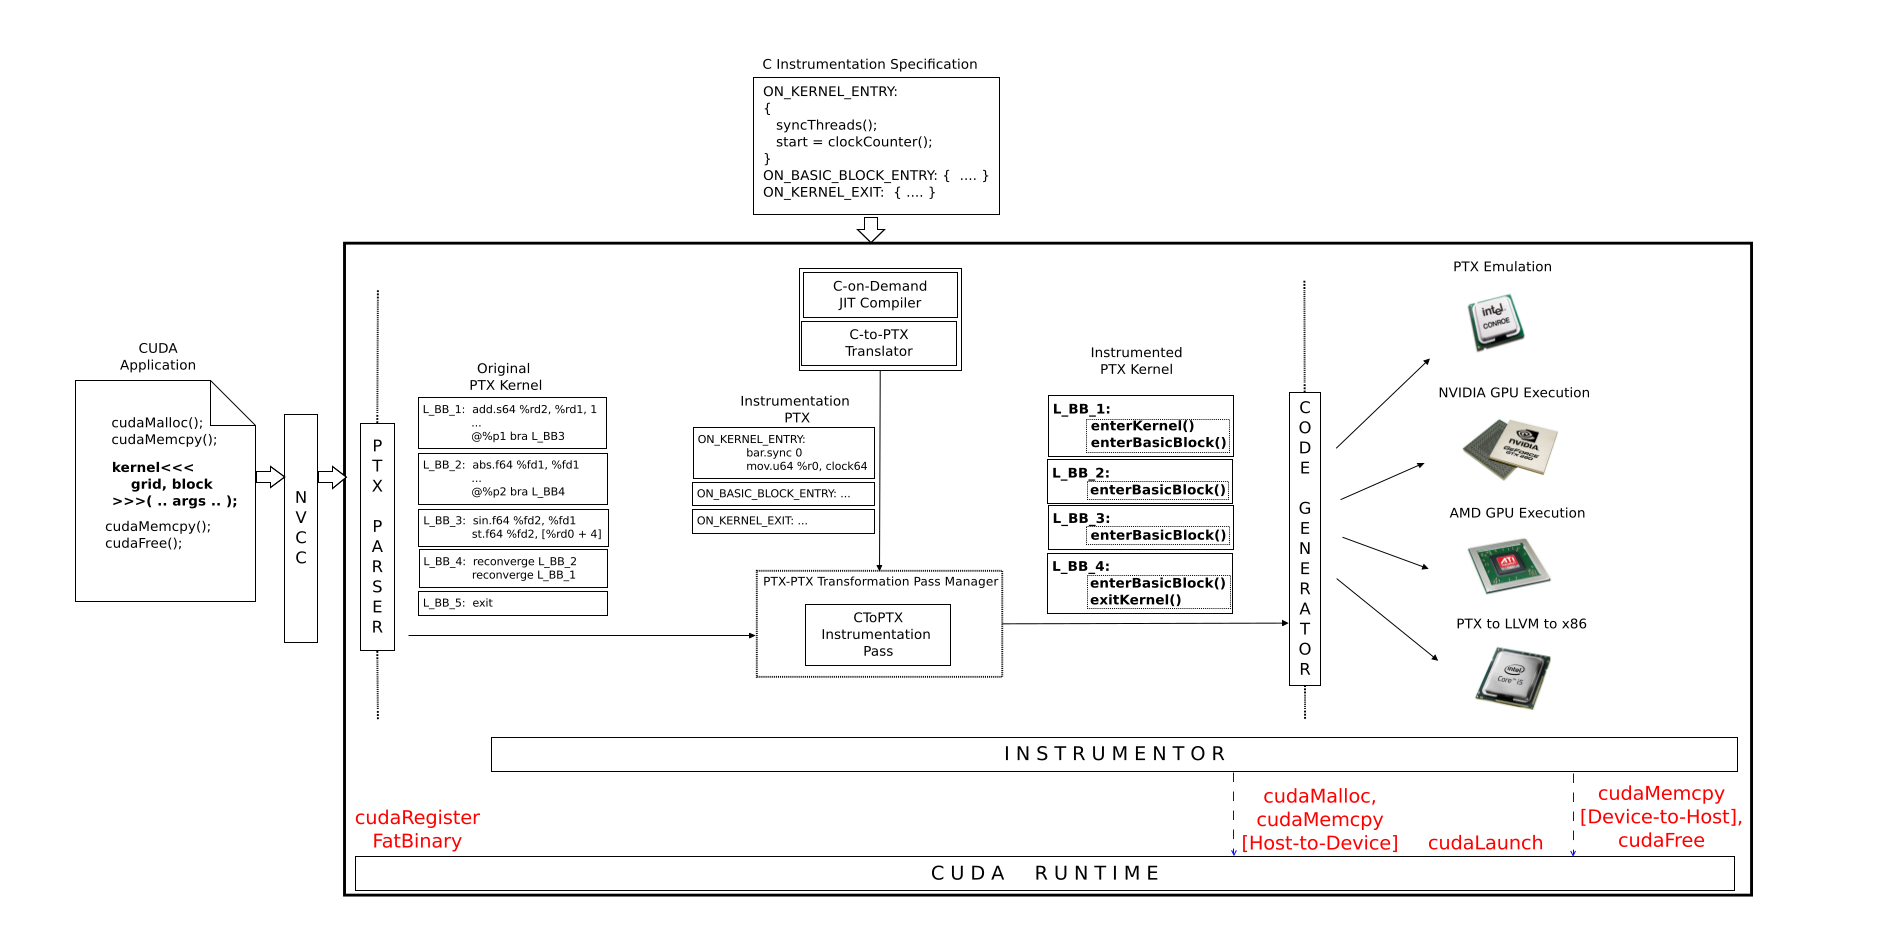
\includegraphics[trim={2.5cm 0 4cm 0},clip,width=\textwidth]{lynx-rt}
	\caption{Lynx framework with all components. The original application is instrumented on PTX level, with code generated by a C-to-PTX JIT from instrumentation specification. Generated data is moved and form the device by the runtime. Image from \cite{Farooqui:2012:LDI:2310660.2310989}}
	\label{lynx-rt}
\end{figure}
%\section{MPI Communication Traces}
%\begin{itemize}
%	\item Not the same because Message Passing != Shared Memory
%	\item Communication Patterns: Rolf Riesen: Paper on Communication Analysis and Patterns, not focussing on special Applications or Architectures. Provides useful metrics to discuss communication
%\end{itemize}
	\chapter{Methodology}\label{methodik}
This chapter explores how GPUs convey information using a shared memory and defines what communication means in the context of this work. Using this definition, the analysis space is described and explored.
\section{GPU Shared Memory Communication}
Other than the explicit communication routines of MPI like send and receive, GPUs convey information implicitly via the global memory on the device. 
The CUDA execution model and the given guarantees can be mapped to the Bulk-Synchronous-Parallel (BSP) bridging model, explained in \ref{sec:bsp}.
\begin{itemize}
	\item \textbf{Computation} is a kernel executed on the GPU. The local components in the model are represented by CTAs on a GPU. Although BSP allows shared memory interactions, CUDA does not, therefore  each CTA is processing it's own workload without the ability to directly interact with other CTAs. 
	\item \textbf{Communication} in this step data generated in the computation step is placed in a location where it can be accessed by a component using the data in a following superstep. For GPUs this location is 
	global memory, because it is modifiable by a kernel during execution and it's modifications persist beyond kernel completion boundaries. In other words, global memory is a memory area allowing visible side-effects
	of a kernel execution.
	\item \textbf{Synchronization} on the GPU happens implicitly by the kernel completion boundary. It guarantees visibility of all global memory operations by the kernel. This implies that follow-up supersteps can see the memory modifications. Just as the barrier in BSP makes sure the communication step
	has been completed by all processors. Partial synchronization is only possble if kernels are members of different streams.
\end{itemize} 
 Not all of the side-effects mentioned above however, can be classified as communication. In the context of this work, communication is data that is written to global memory by one thread and read by another. The CUDA consistency model allows reliable communication only across kernel completion boundaries. We only consider elements that are communicated reliably.

\begin{figure}[t]
	\centering
	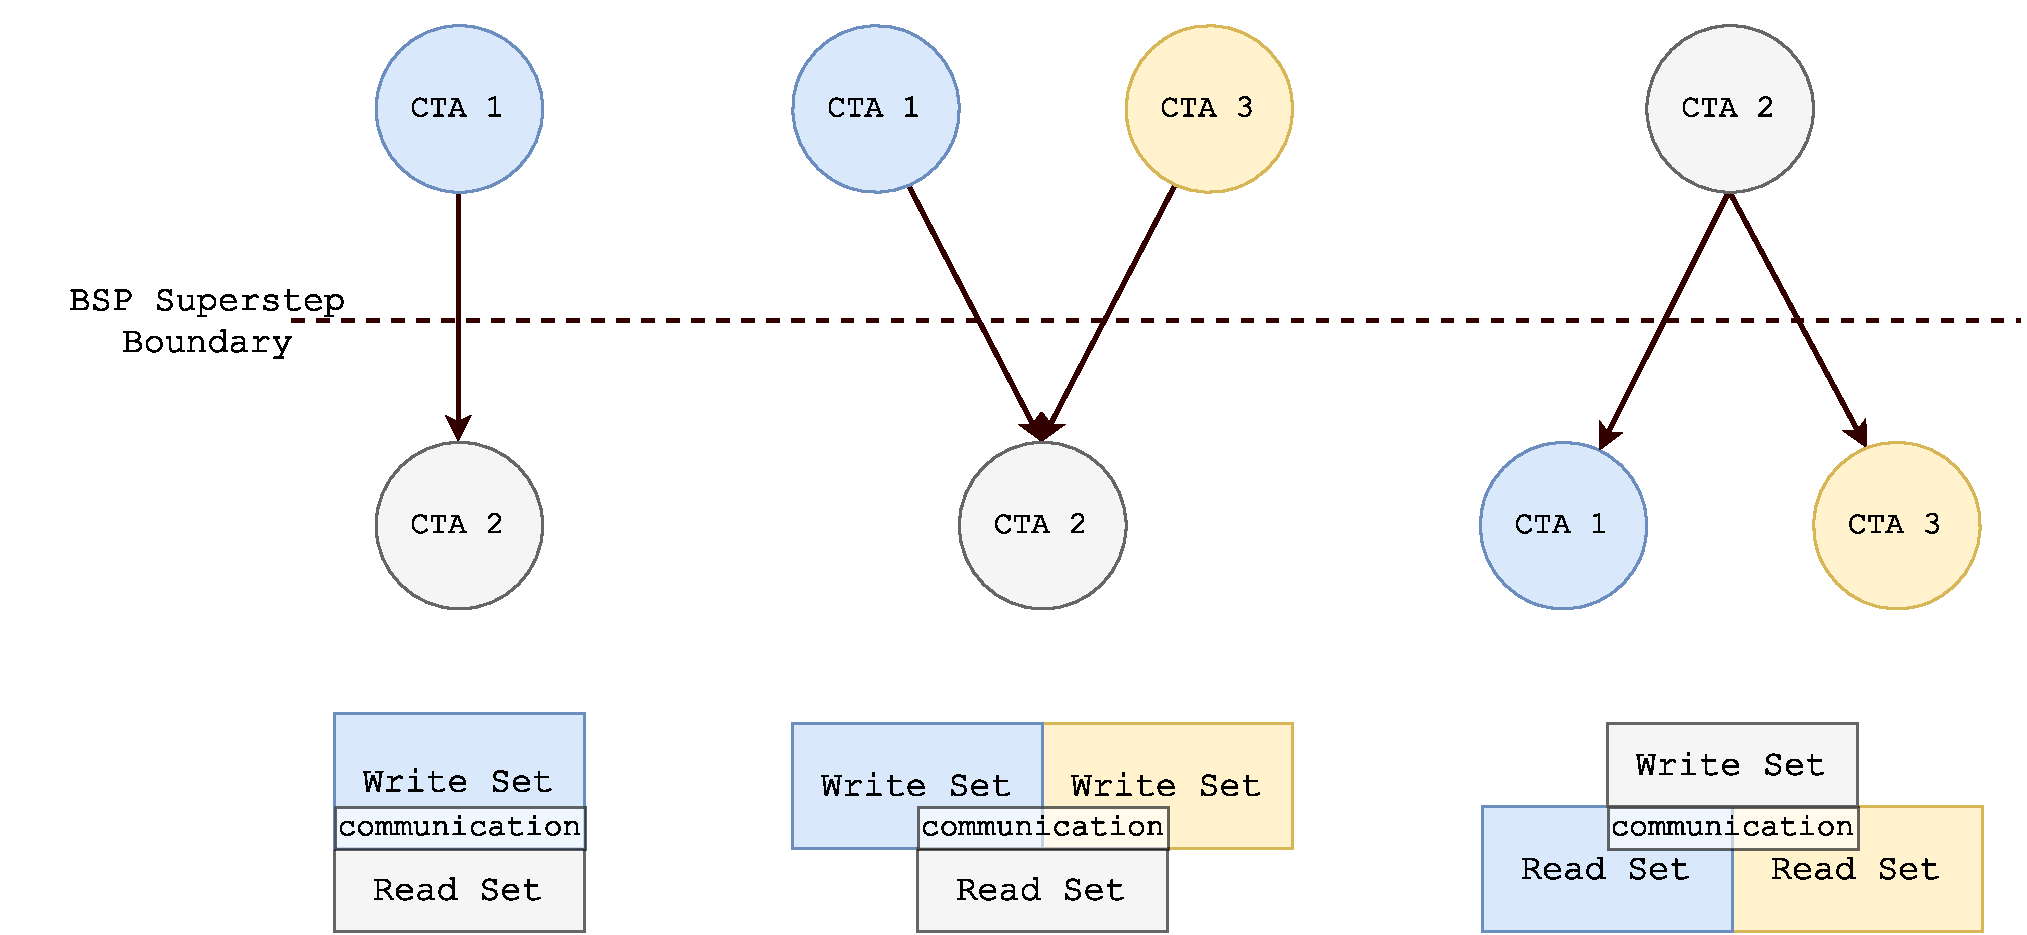
\includegraphics[width=\textwidth]{gpu-comm}
	\caption[CTA Communication]{Communication of CTAs across a BSP superstep boundary, and how this corresponds to read and write sets 
	of sinks and sources. Edges are logical representations of communication, which is actually the overlap of write and read addresses in different BSP supersteps. Different colors represent different sink/source entities.}
	\label{gpu-comm}
\end{figure} 
To exemplify the definition above, figure \ref{gpu-comm} shows how communication between CTAs across a 
BSP superstep boundary translates to overlaps of write- and read-sets. The nodes above the superstep boundary are data sources, the nodes below sinks. The accumulated edge-weight is the size of the 
overlapping area in the write- and read-sets. The left-most graph is a simple point-to-point connection, the middle one resembles a gather collective and the right-most graph can be a scatter or multicast, depending on the overlap. More on collectives in \ref{collectives}.
This representation works for all levels of granularity in the hierarchy of the GPU execution model, from a single thread to an application using multiple kernels and streams.

\section{Analysis Space Exploration}

The analysis space for this work can be separated into spatial and temporal dimensions. The spatial dimension includes the layered hierarchy of threads, CTAs and Kernels. Each hierarchy layer is the superset of the underlying layers. For example, the total data volume written by a kernel is the sum of all its CTA's writes. 
Granularity determines how detailed the spatial dimension is analysed.
The coarsest granularity would be a complete application with multiple kernels and iterations, and the finest a single thread. For this work however, CTAs are used as the finest granularity. The spatial dimension can help characterize an application, but by itself cannot describe communication.

The temporal dimensions describes the series of executed BSP supersteps. Without this dimension, there is no communication to analyse, because by our definition, communication requires at least two subsequent supersteps.
Again, different granularity can be applied to the analysis. Granularity refines, as the term to describe the analysis in this dimension becomes more and more specific. The coarsest granularity ignores individual kernels and exclusively looks at the interaction between the existing supersteps. At finer granularities, the number of supersteps in the analysis may change, because only the interaction of two distinct kernels $k1$ and $k2$ across time $t$ is of interest.

\subsection{Analysis Methods}\label{methodik:methods}
Based on the dimensions and granularities, different tiers for the analysis can be defined.
\begin{enumerate}[I]
	\item Kernel behaviour across all supersteps
	\item Kernel interactions across two supersteps
	\item CTA interactions across two supersteps
\end{enumerate}
The analysis tries to avoid averaging and instead use aggregated values and relational metrics for comparison and analysis.


\subsection{Caveats}\label{collectives}
\begin{itemize}
	\item This work uses CTAs as the fundamental entities of communication source and sink, not threads.
	\item While MPI offers collective communication with clear definitions such as scatter, gather or multicast, the implicit memory communication of GPUs often can not be categorized as clearly. However the in- and out-degree of a communication entity might indicate tendencies towards a certain kind of collective.
	For the sake of the analysis, each collective communication ($\textrm{\{n:1\} \{1:n\} or \{n:n\}} $) can be viewed as a set of point-to-point communications, happening at the same time.
	\item  A kernel execution is a BSP superstep and is serialized with follow-up kernel iterations, or supersteps. Each stream is treated as
	an individual sequence of BSP supersteps during the execution. Stream interactions can be recreated in the follow-up analysis.
	\item Communication across BSP steps, honouring the guarantees CUDA's execution model gives, is not bound to any timing or ordering during the execution of a single compute kernel. Negative performance impacts by the instrumentation are therefore tolerated, 
	because in a well-written program the negative impact does not impede the correctness.
\end{itemize}
	\chapter{Dynamic Instrumentation Using Code Analysis And Transformation For Detailed GPU Communication Analysis}
This chapter describes in detail how the instrumentation works and will do so in the same order of steps as how an application is processed to generate traces.
First, the original application is instrumented on AST and LLVM IR level for tracing, then the data is generated on the GPU during the execution and transported to the host where it is stored in the trace file.


Disclaimer: No Libraries calls in code possible!

Figure \ref{compilestack} shows the necessary steps to add tracing to an application. The first step performs source-to-source compilation that augments the following kinds of statements in the original source with instructions required
for tracing.
\begin{itemize}
	\item Kernel Declarations
	\item Kernel Definitions
	\item Kernel calls
	\item \verb|__device__| function declaration
	\item \verb|__device__| function definitions
	\item \verb|__device__| Function calls inside a Kernel
\end{itemize}
These augmentations have to be performed for each file that contains either of the above statements individually because the process generated new files
rather than overwriting the original source files. More details on the matter in section \ref{sec:impl:clang}

The next step is the introduction to 

Then explain how the tracing is introduced into the application
\begin{enumerate}
	\item Generate object files from augmented source files and insert tracing with LLVM Plugin:
	\item Linking
\end{enumerate}


\section{Source to Source Compilation in CLang}\label{sec:impl:clang}
\begin{itemize}
	\item User has to know which files need augmentation
	\item Augmentation of one file at a time, since out-of-place code transformation is performed
	\item Working in Clang AST
	\item Find all places in the code that need Augmentation:
	\begin{enumerate}
		\item Kernel Definition: Add set of arguments used for tracing
		\item Kernel Calls: Add arguments used for tracing
		\item Include File offering the tracing utils
	\end{enumerate}
\end{itemize}
\section{Code Transformation in LLVM}
\begin{enumerate}
	\item Pointer Analysis: Proof Global Memory "origin" of Pointer used in Memory operations (Load, Store, Atomics): Context Sensitive, Spase Flow Analysis in SSA, 3 Element Lattice Problemspace, Monotonic Transfer function, Pathological Cases (PhiNodes/Certain Functions)
	\item Versioning: Replicate Device Functions with ambiguous memory spaces
	\item Code Transformation: Insert Instructions used for tracing
	\item Technical Limitations (module boundaries) 
\end{enumerate}

\section{Tracing Process}
	Many applications have non-deterministic executions, eg no fixed number of kernel calls because of varying input data. Examples for is the Breadth-First-Search, which is heavily depending on the underlying graph's structure or PDE solvers which iterate until the
	convergence condition is reached by the residual. Because of this, a static buffer that is simply filled up does no suffice for reliable tracing.
	
	Therefore a producer-consumer between GPU and host is used that ensures the application never runs out of trace-buffer space.
	The buffer containing the generated data is host-mapped memory, which is separated into several bins. The bins are used to reduced
	pressure on the memory system that is generated by the atomic accesses of the producer-consumer setup.
	
	\subsection{Warp-Scope Producer}
	This section focusses on the producer that is running on the device, making sure that data is only written if there space left
	in a buffer. The producer-consumer setup uses a head and a tail index to handle reservation of buffer space and write acknowledgements. Listing \ref{prod-cons} shows the pseudo-algorithm that is performed by the producer.
	\begin{lstlisting}[style=perl]
while((ackIndex > maxIndex) or (res = atomicAdd(resIndex, increment) > maxIndex)) 
buffer[res] = traceData
atomicAdd(ackIndex, increment)
	\end{lstlisting}\label{prod-cons}
	The first line makes sure, that the buffer still has enough space, otherwise the loop waits until the buffer is evacuated by the host. This simplified version 
	
	
	This happens on a warp scope to prevent deadlocks during indices fetching caused by branch divergence inside of warps.
	The deadlock happens because of how GPU handle warp scheduling and and branch divergence. If a branch happens inside a warp, all member threads of this warp execute both branches, but the group of members that should be inactive is masked out.
	
	\subsection{Host Consumer}
	\subsection{Stream Handling}
\begin{itemize}
	\item General Tracing Setup
	\item Producing Data on the Device: Handling Indices on a Warp Scope
	\item Consuming data on the host side
	\item Handling Streams
\end{itemize}



	\chapter{Evaluation and Analysis of GPU Communication}\label{eval}
This chapter analyses the traces generated with the technique described in chapter \ref{chap:impl}. The analysis is sectioned into several tiers, as described in \ref{methodik:methods}.\\


\section{Evaluated Applications}
The evaluated application are listed in table \ref{eval-apps}. The applications are selected to represent typical problem Domains in scientific computing. 
\begin{table}[h]
	\centering
\begin{tabular}{|l|c|c|c|c|}
	\hline 
	\textbf{Application} & \textbf{Source} & \textbf{Domain} & \textbf{Abbreviation} &\textbf{Problem Size} \\ 
	\hline 

%	\hline 
	Hotspot 2D & Rodinia & Structured Grid 2D & hs2d & 512x512, t = 10\\ 
%	\hline 
	Hotspot 3D & Rodinia & Structured Grid 3D & hs3d& 512x512x8, t = 10\\ 
%	\hline 
	Histogram64 & CUDA SDK & Histogram & hist& 64MB into 64 Bins\\ 
	NBody & ZiTi CEG & Nbody & nbody& 512 Bodies, t = 5\\ 
	Pathfinder & Rodinia & Shortest Path & path& 100000x100x20\\ 
%	\hline 
	Breadth First Seach & Rodinia & Graph Processing & bfs& $10^{6}$ Nodes\\ 
%	\hline 

	\hline 
\end{tabular} 
\caption{Application used for communication evaluation}
\label{eval-apps}
\end{table}
\textit{Hist}, \textit{hs2d}, \textit{hs3d} and \textit{nbody} are regular applications, where each CTA only operates within his data region. \textit{BFS} and \textit{path} contain irregularity, as the execution is  dynamic and the behaviour is depended on the input data.
\section{Tier I Analysis}
\subsection{Total Data Volume and Communication Fraction}
 Figure \ref{com-ratio} directly compares the total data volume of loads and stores of and how much of the write volume is involved in communication. At least 30\% of any application's writes is accessed by another CTA or another kernel in following iterations. As expected, loads exceed the stores by at least a single order of magnitude.

\textit{Nbody} and \textit{hist} show a very high ratio of communication, because \textit{nbody} is an $n$-to-$n$ problem and the histogram algorithm reduces a problem into bins, only using on the data generated in the preceding step. The irregular applications, \textit{bfs} and \textit{path}, communicate less data compared to the four regular applications.

Against initial expectations,  \textit{hs2d} and \textit{hs3d} show almost 50\% communication ration. The reason is, \textit{hs2d} uses deep halos which increase the number of transferred bytes between iterations. \textit{Hs3d} exchanges the complete $z$-dimension across iterations. 


\begin{figure}[t]
	\centering
	\includegraphics[width=\textwidth]{../../../Global-Memory-Tracing/memtrace-pass/plots/write-com-ratio}
	\caption{Total data volume and ratio of communication to total of all writes.}
	\label{com-ratio}
\end{figure}
\subsection{Transfer Size CDF}
Figure \ref{fig:CDF} shows the cumulative distribution functions (CDF) plots for each application. The CDF shows the cumulative probability of a transfer size between two CTAs to occur during the execution. All applications, except \textit{path}, show one or few dominating transfer sizes. The \textit{path} application shows two slopes with linear rising probability for a range of transfer sizes.

The dominant transfer size of \textit{bfs} is caused by the frontier array, used to communicate across graph segments. The \textit{hist} has one transfer size, because only one uniform kind of transfer happens in this application. This is also true for \textit{nbody}. The steps in \textit{hs2d} and \textit{hs3d} are caused by the problem space borders in the calculation

\begin{figure}[t]
%	\begin{subfigure}[b]{0.45\textwidth}
%		\includegraphics[width=1\linewidth]{../../../Global-Memory-Tracing/memtrace-pass/plots/cdf/bfs}
%		\caption{BFS}
%		\label{fig:cfd-bfs}
%	\end{subfigure}
%	\begin{subfigure}[b]{0.45\textwidth}
%		\includegraphics[width=1\linewidth]{../../../Global-Memory-Tracing/memtrace-pass/plots/cdf/hist}
%		\caption{Histogram}
%		\label{fig:density-hist}
%	\end{subfigure}
%	\begin{subfigure}[b]{0.45\textwidth}
%		\includegraphics[width=1\linewidth]{../../../Global-Memory-Tracing/memtrace-pass/plots/cdf/hs2d}
%		\caption{Hotspot 2D}
%		\label{fig:cfd-hs2d}
%	\end{subfigure}
%	\begin{subfigure}[b]{0.45\textwidth}
%		\includegraphics[width=1\linewidth]{../../../Global-Memory-Tracing/memtrace-pass/plots/cdf/hs3d}
%		\caption{Hotspot 3D}
%		\label{fig:cfd-hs3d}
%	\end{subfigure}
%	\begin{subfigure}[b]{0.45\textwidth}
%		\includegraphics[width=1\linewidth]{../../../Global-Memory-Tracing/memtrace-pass/plots/cdf/path}
%		\caption{Pathfinder}
%		\label{fig:cfd-path}
%	\end{subfigure}
%	%add desired spacing between images, e. g. ~, \quad, \qquad, \hfill etc. 
%	%(or a blank line to force the subfigure onto a new line)
%	\hfill
%	\begin{subfigure}[b]{0.45\textwidth}
%		\includegraphics[width=1\linewidth]{../../../Global-Memory-Tracing/memtrace-pass/plots/cdf/nbody}
%		\caption{NBody}
%		\label{fig:cfd-nbody}
%	\end{subfigure}
	\includegraphics[width=\textwidth]{../../../Global-Memory-Tracing/memtrace-pass/plots/combined-cfd}
	\caption{Message Size CDF Plots}
	\label{fig:CDF}
\end{figure}


\subsection{CTA In/Out-Degree}
The in and out degree describe the number  communication partners, separated between incoming and outgoing transfers, for each CTA. Figure \ref{fig:Cta-degree} plots the percentages of selected bins for each application. 

Except for \textit{nbody}, and to a smaller degree \textit{bfs} and \textit{path}, no application performs point-to-point communication. Almost every communication happening is, to some degree, a collective communication.

Most applications show low variance of in- and out-degree, and few communication partners. \textit{Bfs} has a high variation because the traversed graphs dictates the communication partners. The partners of \textit{hs2d} are a result of 2D tiling and \textit{hs3d}s partners
dictated by stencil size. Also notable is that although \textit{path} is a dynamic application, the number of communication partners is steady. The in/out-degree of \textit{hist} stems from the two-step process, where each CTA in the second step reads a value from
every CA in the first step.

\begin{figure}[t]
	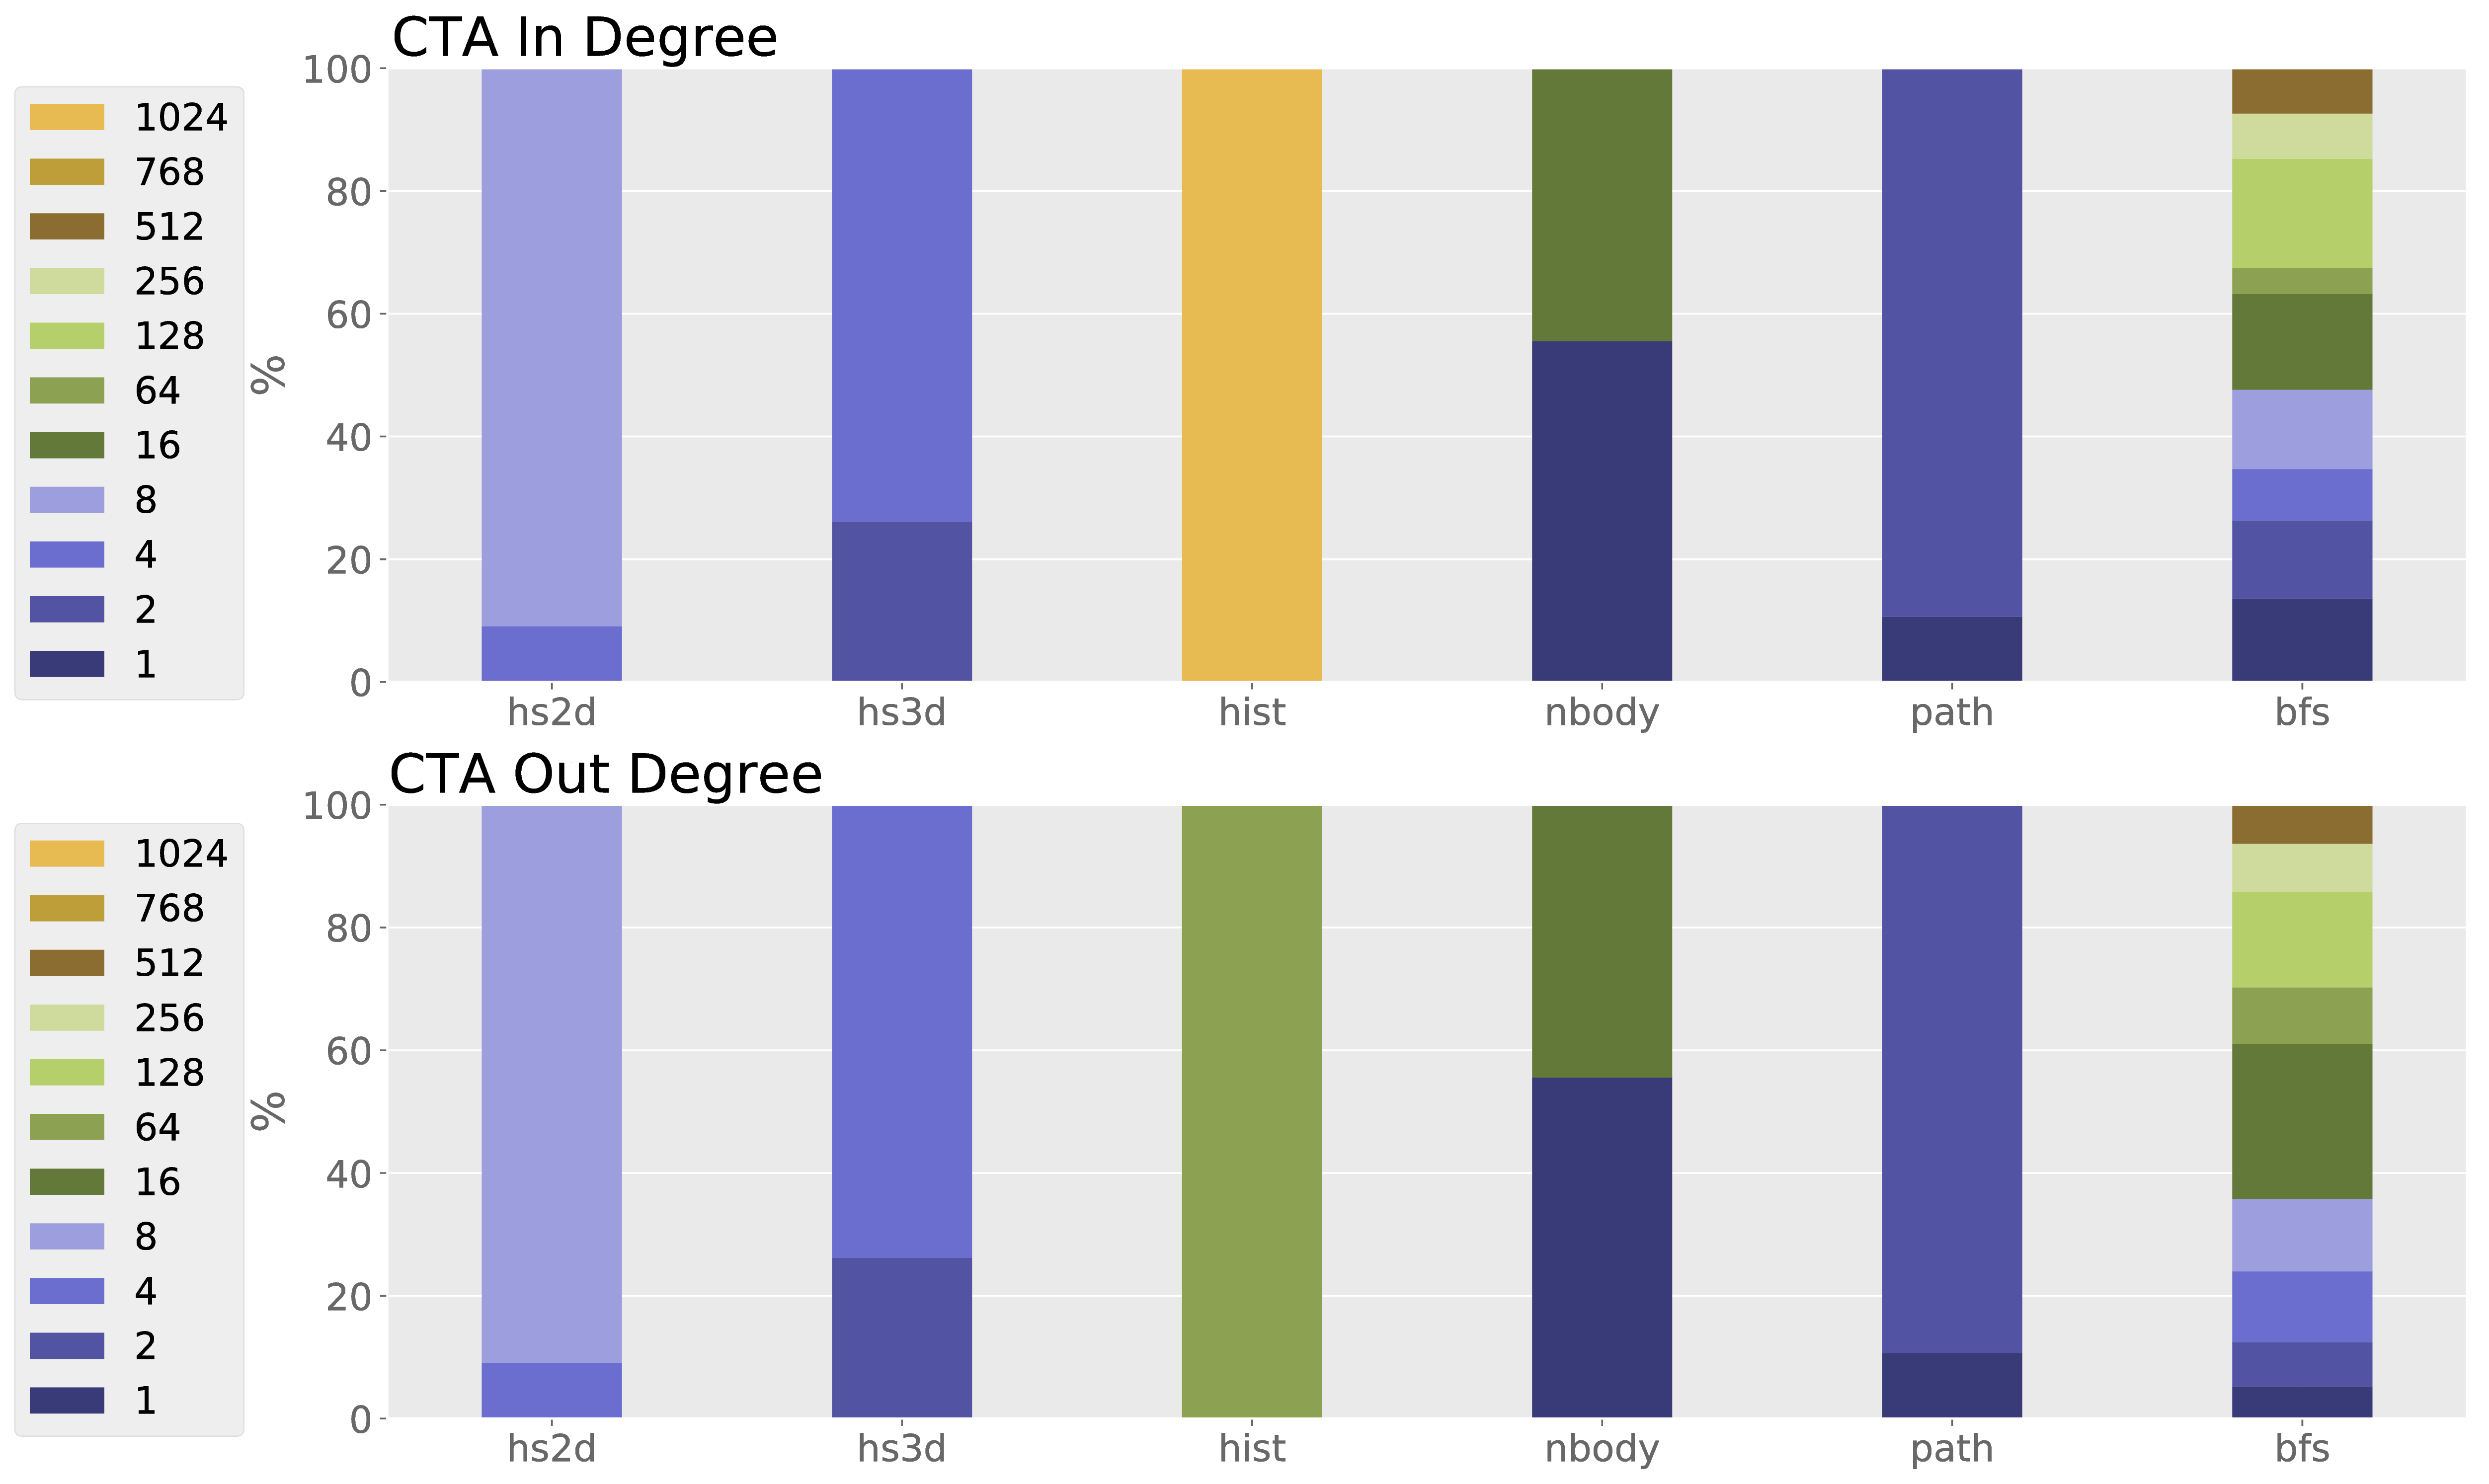
\includegraphics[width=\textwidth]{../../../Global-Memory-Tracing/memtrace-pass/plots/cta-degree}
	\caption{Number of incoming and outgoing communication partners of each CTA}
	\label{fig:Cta-degree}
\end{figure}
\subsection{Bisection Volume}
This metric shows the data volume moved a hypothetical cut in each dimension. The cut creates two equally sized grids. This can help analyse, how well an application scales to multiple GPUs. Because none of analysed application use the $z$-dimension of CTA organisation, only the $x$ and $y$ dimensions are plotted. 

\textit{Hs3d} strikes out, as it clearly shows that a cut in the $y$-dimension would not be favourable. The path algorithm shows a very low bisection volume, making it a good candidate for multi-gpu scaling.
Because of \textit{bfs} very irregular access patterns and high bisection volume and ratio, scaling to multiple GPUs can be challenging. The same goes for \textit{hist} and \textit{nbody}, because they both
perform all-to all communication. The scalability of the stencil applications depends on the problem, stencil and halo size and halo.
\begin{figure}[t]
	\centering
	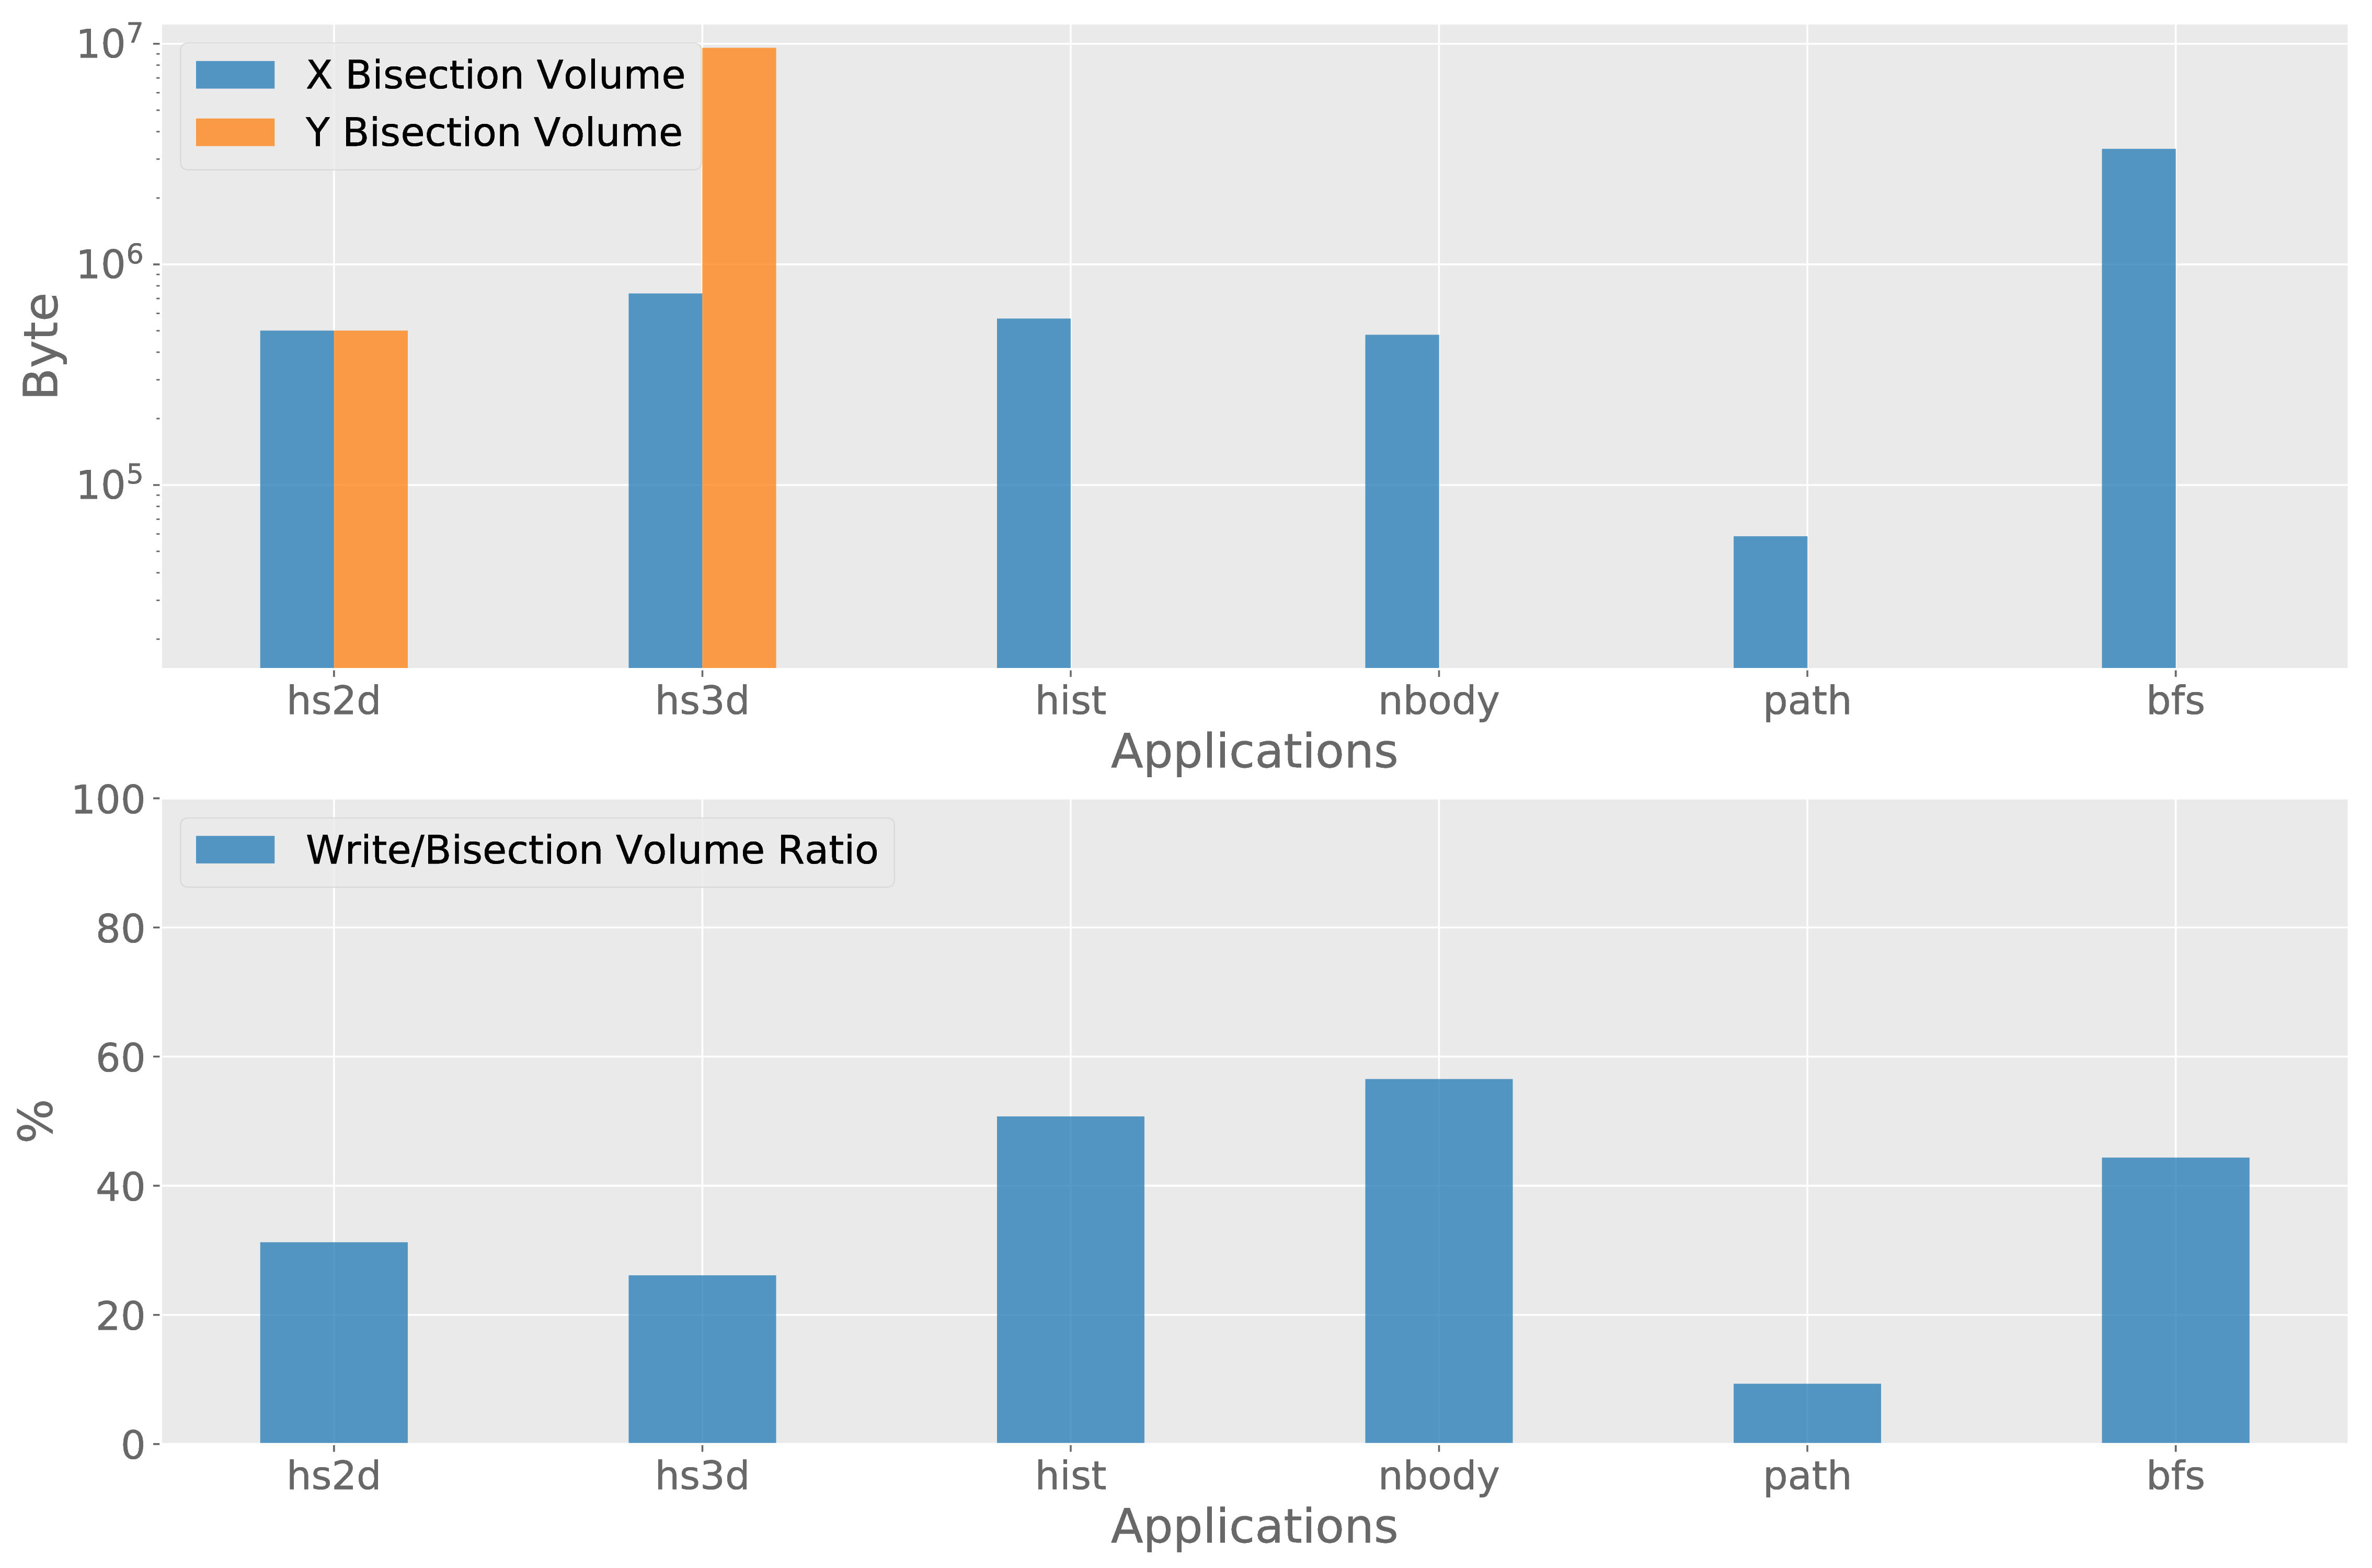
\includegraphics[width=\textwidth]{../../../Global-Memory-Tracing/memtrace-pass/plots/bisection-volume}
	\caption{Total and relative bisection Volume, separated by dimensions}
	\label{bisection-vols}
\end{figure}
\subsection{Communication Stride}
The stride in loads and stores involved in communication can be a critical aspect for performance. Large strides reduce the available memory bandwidth and increase latency. The strides in figure \ref{com-stride} are measured in byte distance, not elements.

The \textit{hist} application shows a large load stride in figure \ref{com-stride}, together with a large in-degree in figure \ref{fig:Cta-degree} suggest a 'gather'-like characteristic. For \textit{hs2d}/\textit{hs3d} we see the expected stride created by the tiling/stencil, accessing multiple rows at once.
The irregular pattern of \textit{bfs} is caused by the frontier array, which is used to communicate between all CTAs. The stride of nbody
is
\begin{figure}[t]
	\centering
	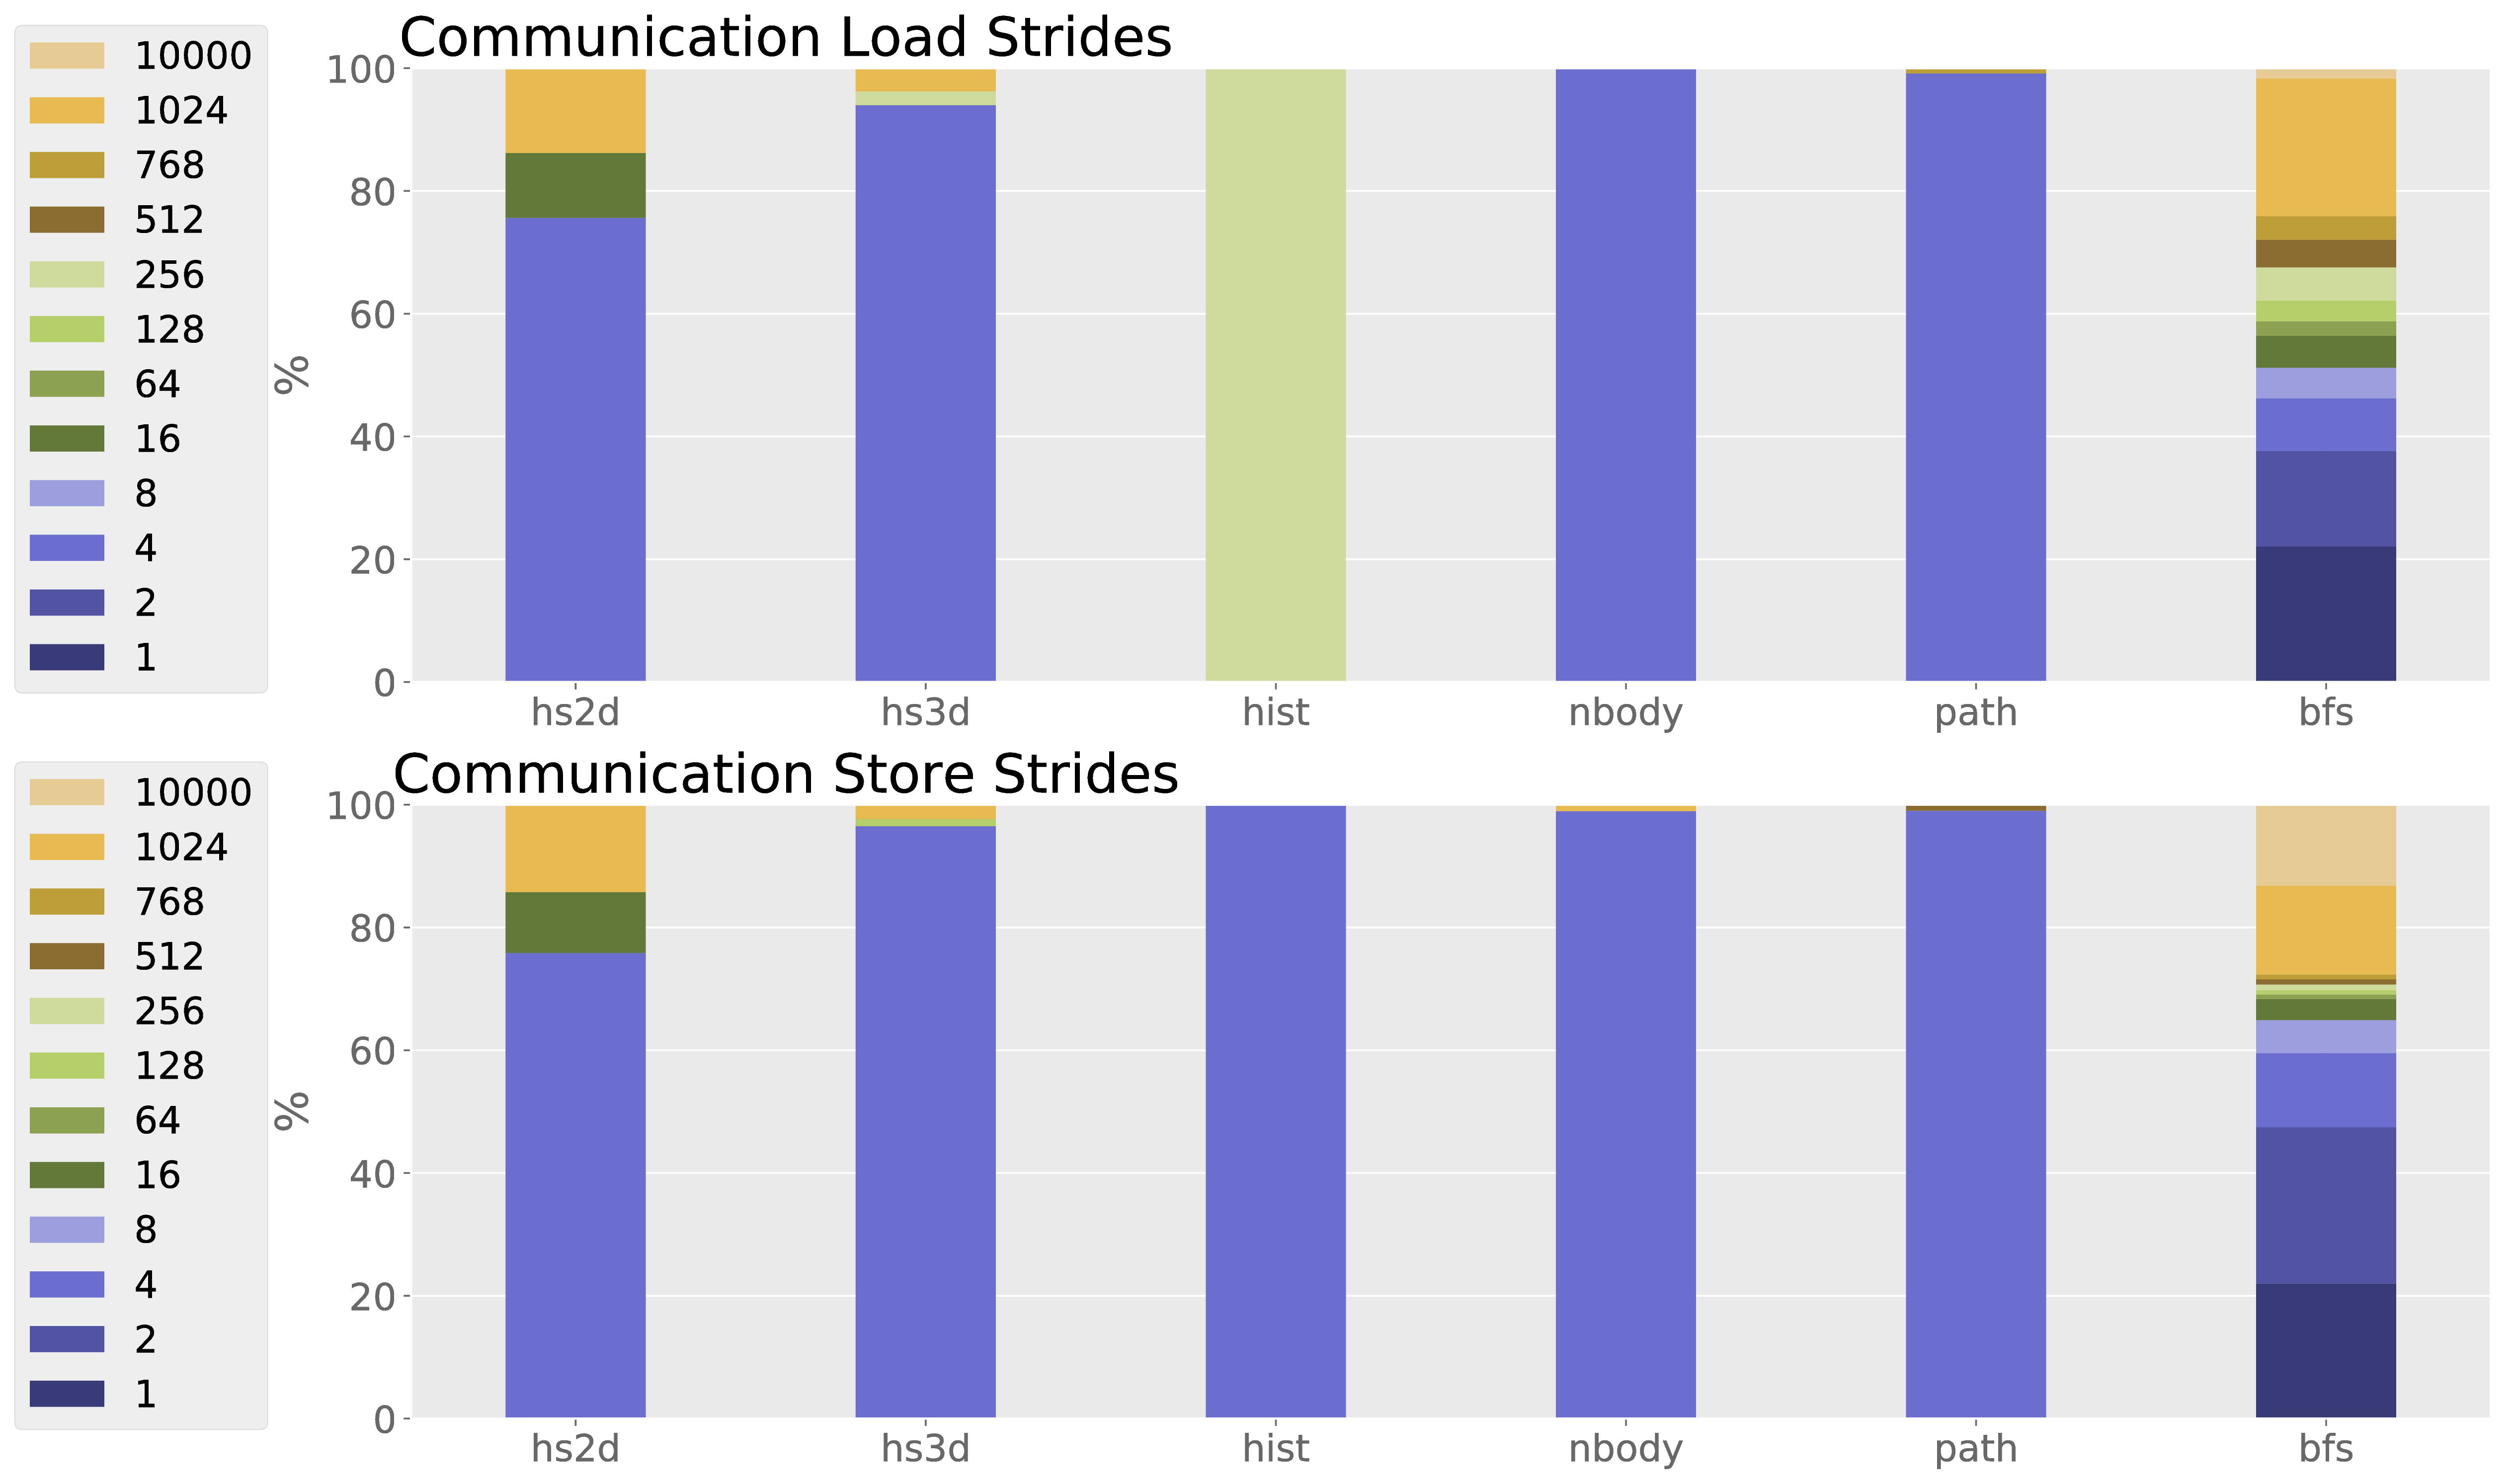
\includegraphics[width=\textwidth]{../../../Global-Memory-Tracing/memtrace-pass/plots/strides}
	\caption{Strides of loads and stores used in communication, by CTA}
	\label{com-stride}
\end{figure}
\subsection{Density Map}
The density plots, sometimes called heatmap, describes the frequency of CTA interaction across BSP supersteps. The x-axis are the CTAs performing writes, the y-axis are the follow-up reads to each write. Different kernels in an application are ignored, and only the CTA ID is used to identify communciation partners. Figure \ref{fig:density-plots} displays a subset of 200 CTAs for each application. The IDs of all CTA are serialized in $x$,$y$,$z$ order, $x$ being the most dominant dimension. 

The regular application show the expected patters. The stencils show communication with their neighbours according to stencil and tiling, \textit{nbody} shows communication with all other CTAs, same as \textit{hist}.

The irregular applications show two very different patters. \textit{Path} has only few partners but the frequency varies significantly. \textit{Bfs} shows two extremes, high frequency with high regularity and low frequency with low regularity.
The first extreme is caused by two kernels alternating during the iterations, where CTAs with the same ID process the same segment of the graph.  Latter is caused by the frontier array, used at the segment borders. A different graph would create the same pattern of the first extreme, but a different pattern of the second extreme.

The \textit{nbody} plot does not show 200 CTAs, as it only used 15 CTAs.

As the CDF plot shows, all applications are dominated by few transfer sizes between CTAs, the patterns in figure \ref{fig:density-plots} would remain largely unchanged if the density was replaced with accumulated data volumes.
\begin{figure}[h!]
	\begin{subfigure}[b]{0.45\textwidth}
		\includegraphics[width=1\linewidth]{../../../Global-Memory-Tracing/memtrace-pass/plots/heatmap/bfs}
		\caption{BFS}
		\label{fig:density-bfs}
	\end{subfigure}
	\begin{subfigure}[b]{0.45\textwidth}
		\includegraphics[width=1\linewidth]{../../../Global-Memory-Tracing/memtrace-pass/plots/heatmap/hist}
		\caption{Histogram}
		\label{fig:density-hist}
	\end{subfigure}
	\begin{subfigure}[b]{0.45\textwidth}
		\includegraphics[width=1\linewidth]{../../../Global-Memory-Tracing/memtrace-pass/plots/heatmap/hs2d}
		\caption{Hotspot 2D}
		\label{fig:density-hs2d}
	\end{subfigure}
	\begin{subfigure}[b]{0.45\textwidth}
		\includegraphics[width=1\linewidth]{../../../Global-Memory-Tracing/memtrace-pass/plots/heatmap/hs3d}
		\caption{Hotspot 3D}
		\label{fig:density-hs3d}
	\end{subfigure}
	\begin{subfigure}[b]{0.45\textwidth}
		\includegraphics[width=1\linewidth]{../../../Global-Memory-Tracing/memtrace-pass/plots/heatmap/path}
		\caption{Pathfinder}
		\label{fig:density-path}
	\end{subfigure}
	%add desired spacing between images, e. g. ~, \quad, \qquad, \hfill etc. 
	%(or a blank line to force the subfigure onto a new line)
	\hfill
	\begin{subfigure}[b]{0.45\textwidth}
		\includegraphics[width=1\linewidth]{../../../Global-Memory-Tracing/memtrace-pass/plots/heatmap/nbody}
		\caption{NBody}
		\label{fig:density-nbody}
	\end{subfigure}
	\caption{Transfer Density Plots}
	\label{fig:density-plots}
\end{figure}
\\\\\\\\\
\section{Tier II Analysis}
\subsection{Kernel communication Evolution}
This analysis if figure \ref{trans-ratio} shows how the data volumes change across supersteps. It is separated into loads and stores. Loads start at superstep one because as to our definition of communication, there can be no load that is part
of communication during the first superstep. Stores are not displayed in the last iteration, because the last store of an application is no communication.

The graph is to read as such: Stores happened in this superstep and are readable in the next. Loads read data from the preceding superstep. CTA in- and out degree analysis showed, every communication is happening in a collective environment. This means that there is no simple single writer, single reader matching across supersteps, which is the reason loads and stores are separated in this graphs.

As expects, the data of all regular applications follow a pattern, while the ones on irregular applications do not. The stencils do not
vary volumes, because every iteration performs exactly the same task. Because each CTA only updates
it's own set of bodies, \textit{nbody} has constant store volumes. The load volume of every other iteration accesses all bodies, creating the zig-zag pattern.
\begin{figure}[h!]
	\centering
	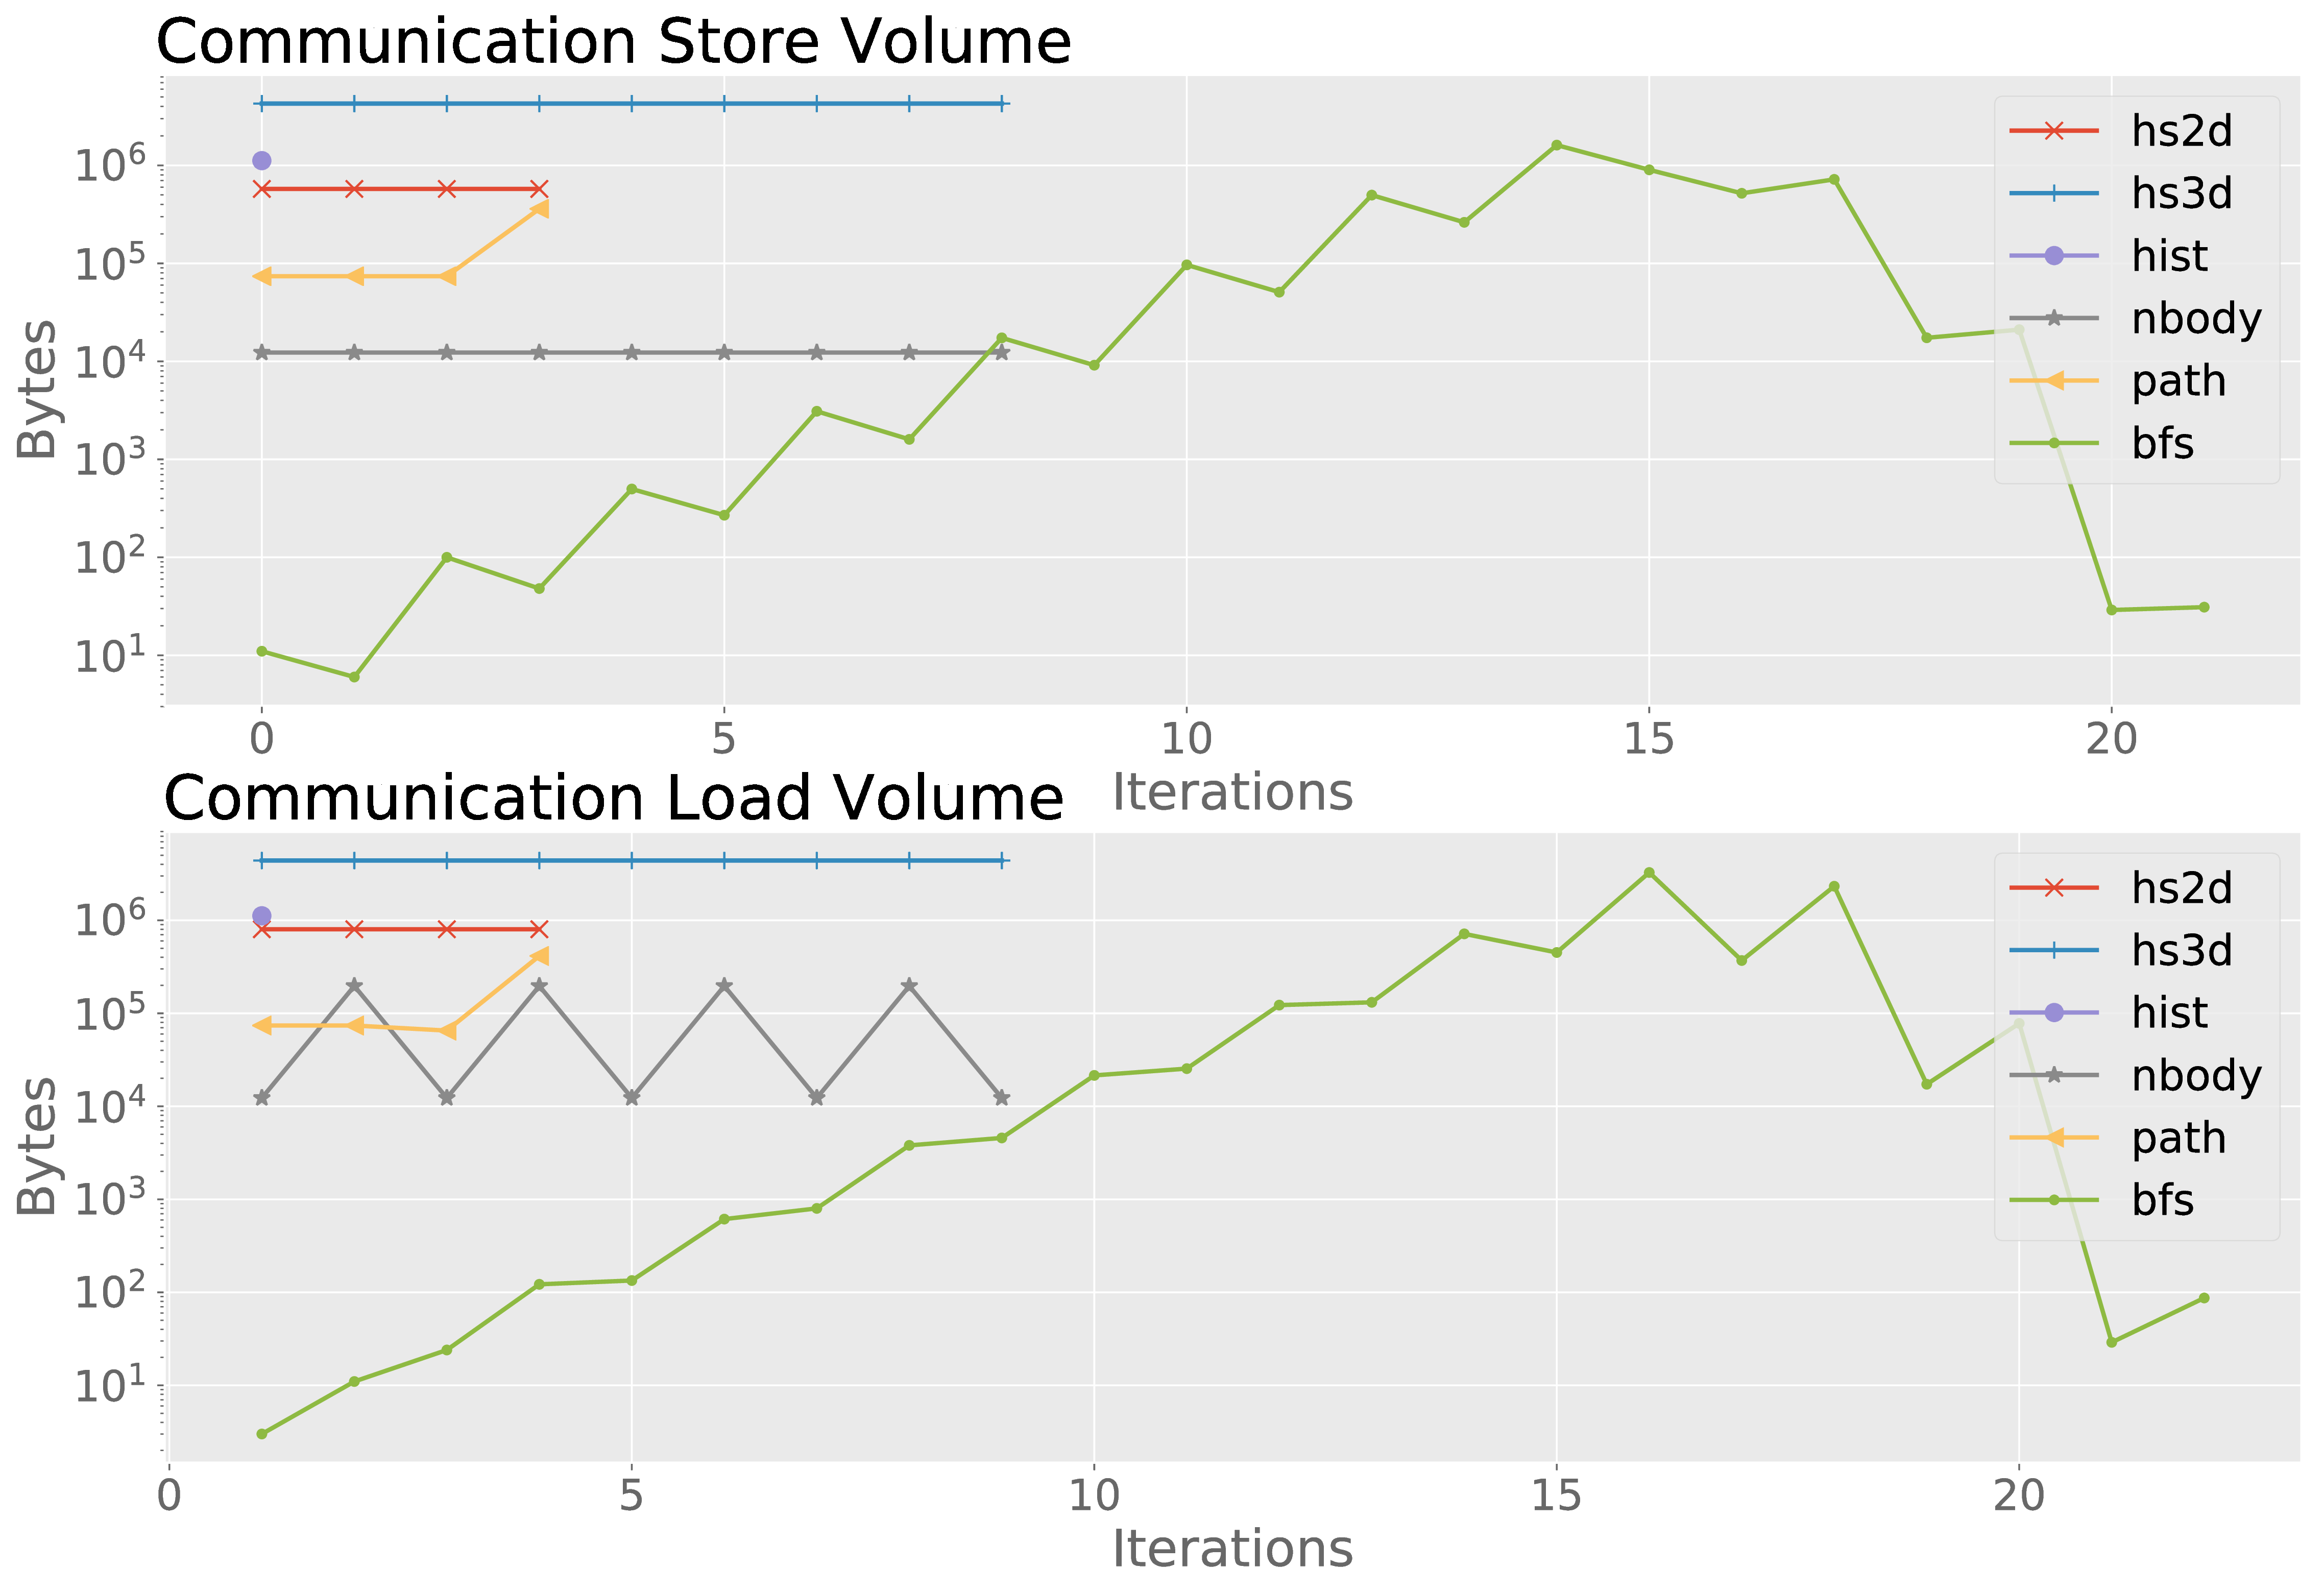
\includegraphics[width=\textwidth]{../../../Global-Memory-Tracing/memtrace-pass/plots/transmission-ratio}
	\caption{Volume of communication loads and stores in each iteration}
	\label{trans-ratio}
\end{figure}
\subsection{Superstep Distance}
This metric measures the volume of data transferred, but takes into account the number of supersteps distance between the store and the subsequent load. Only \textit{bfs} shows this behaviour,
figure \ref{trans-distance} shows only the volume for this application. The distance describes the number
of supersteps, or kernel launches, happening before written data is read by a CTA. A distance of zero means, the directly succeeding kernel reads the data.

Read operations in different supersteps can reference the same write, therefore the volumes are not exclusive.
As an example, a subset of distance zero might very well be included in more distant reads.
\begin{figure}[t]
	\centering
	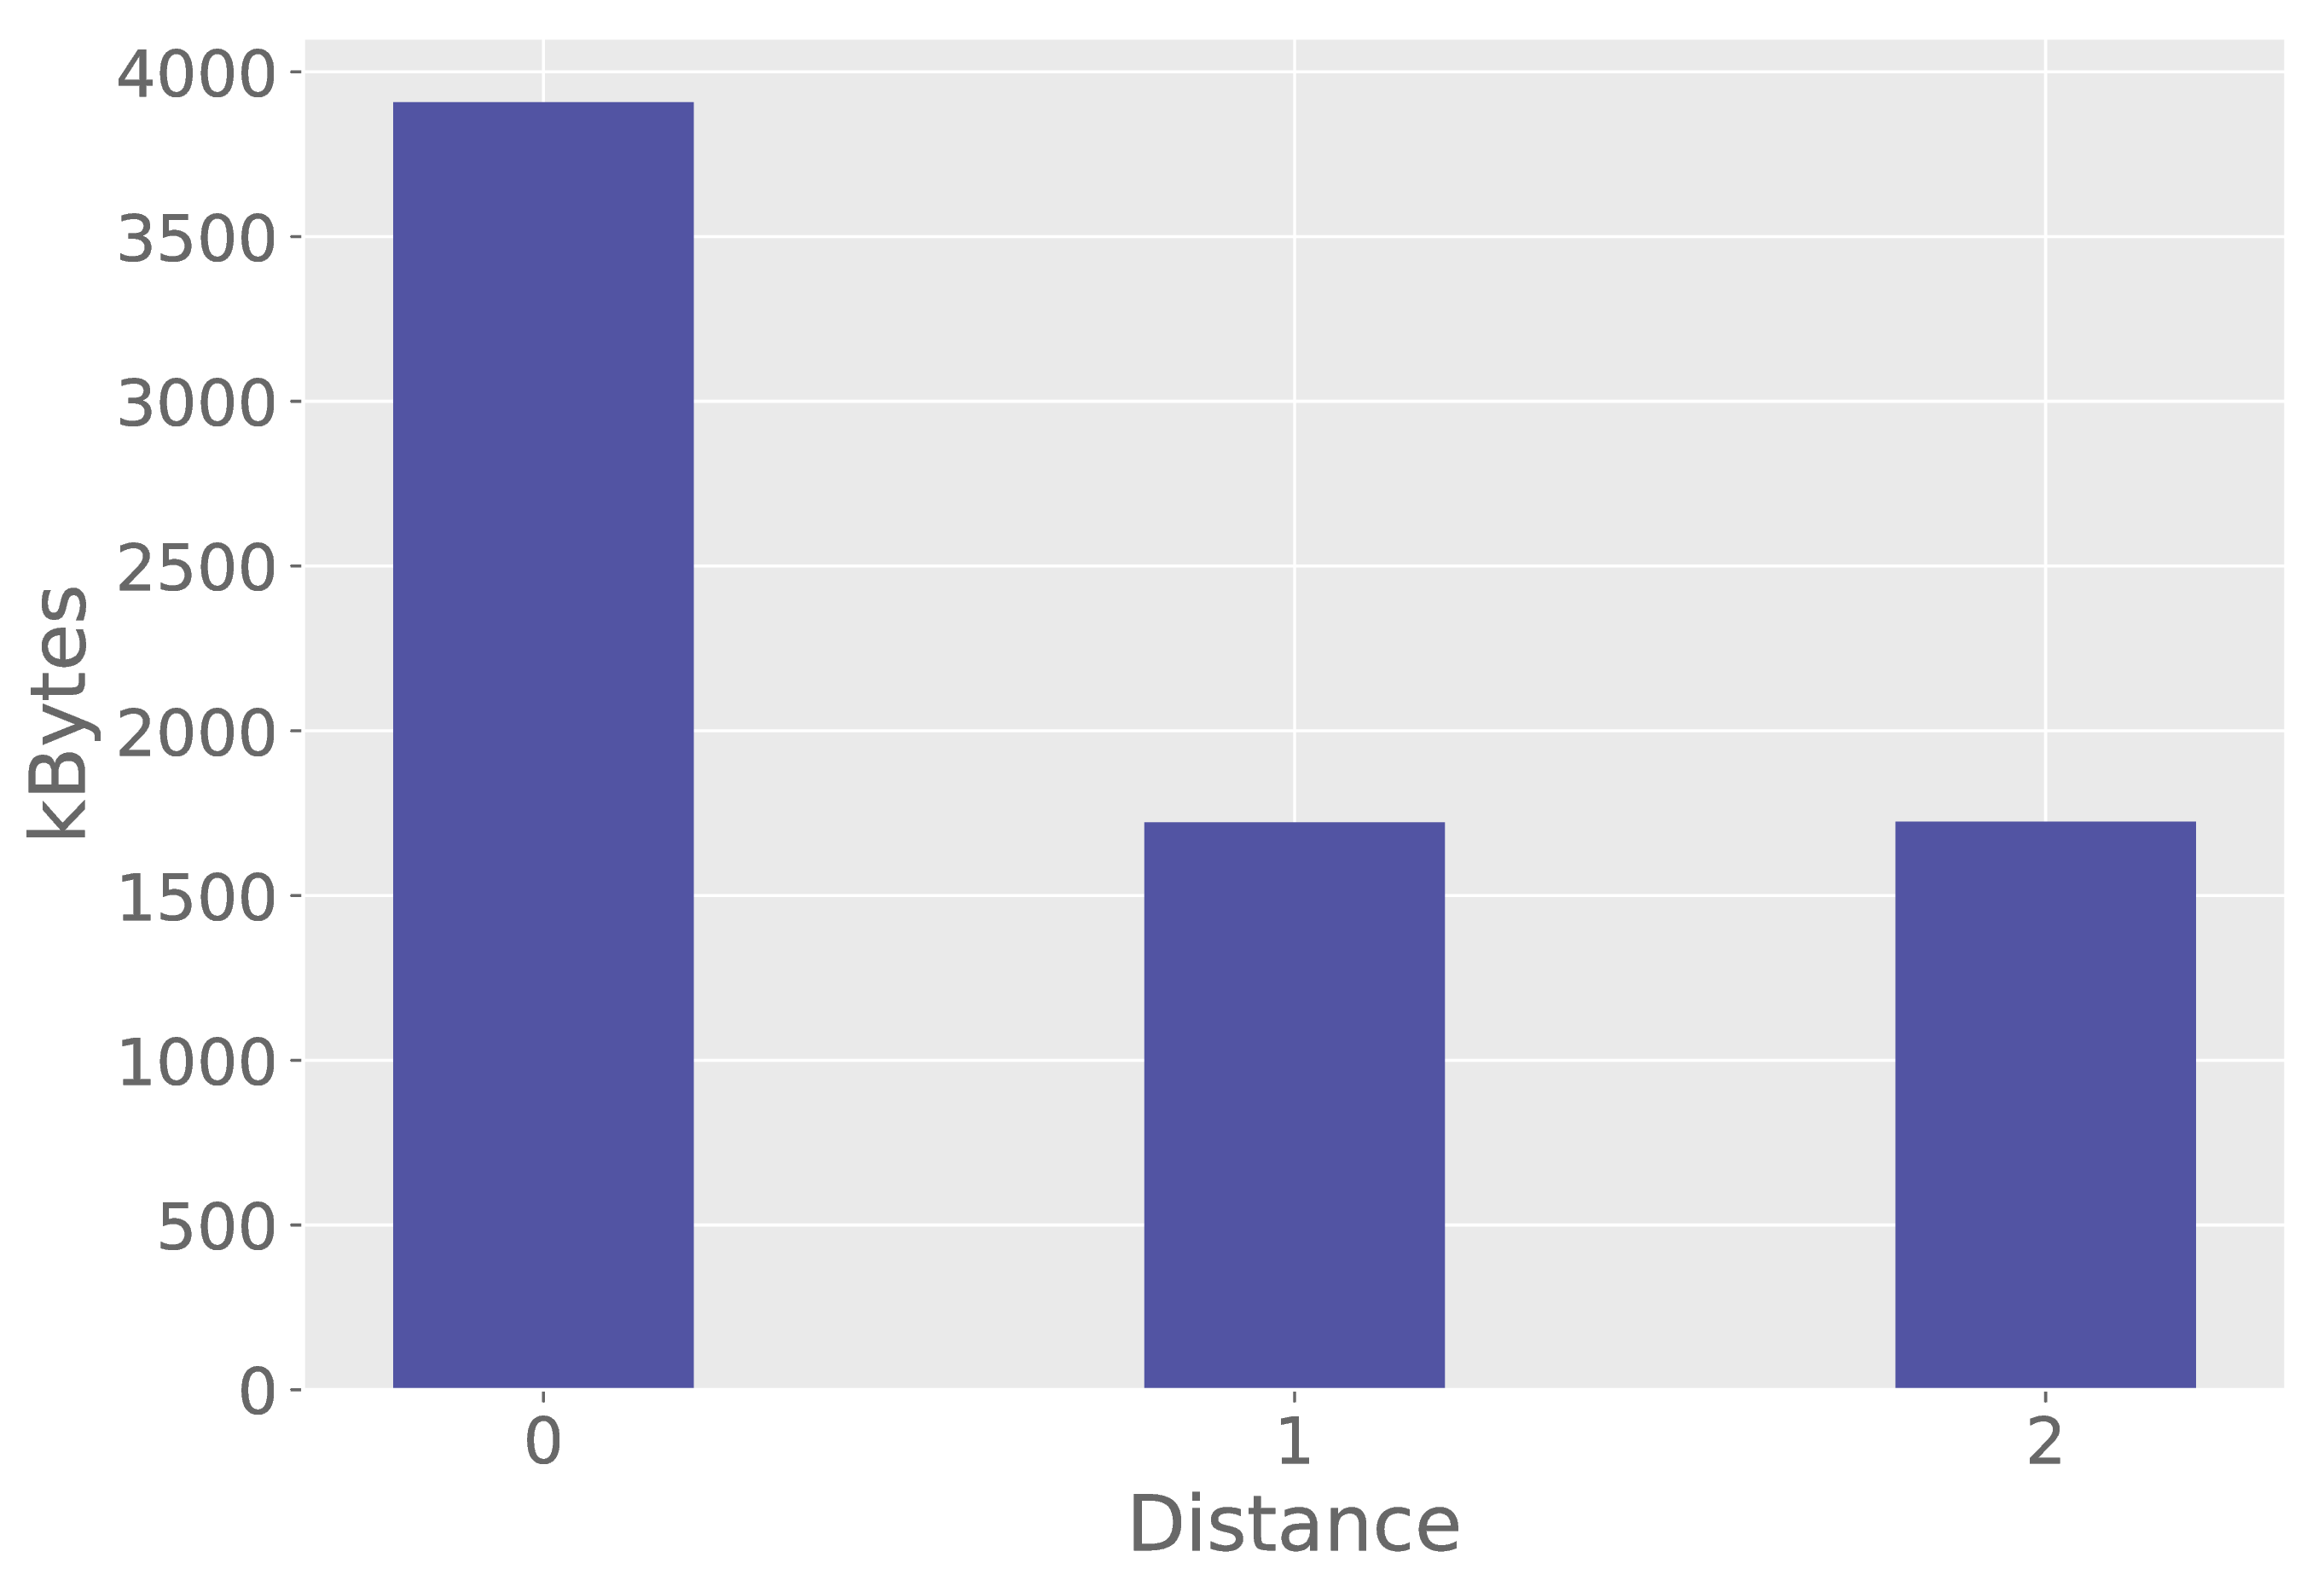
\includegraphics[height=0.3\textheight]{../../../Global-Memory-Tracing/memtrace-pass/plots/distances}
	\caption{Volume of communication for \textit{bfs} application, separated by superstep distance.}
	\label{trans-distance}
\end{figure}
\section{Tier III Analysis}

\subsection{CTA connectivity evolution}
As shown in figure \ref{fig:Cta-degree}, most applications have a steady number incoming and outgoing connections. Figure \ref{philandering} shows how the mean number of outgoing communication partners changes over time, including the standard deviation. 

The large fluctuation of \textit{nbody} can be explained with two alternating kernels, one kernel accesses only it's own set of bodies, while the other kernel accesses all bodies, which increases the out-degree. Because \textit{hist} consists of only two steps, it is represented by single value. Both \textit{path} and \textit{bfs} show stronger fluctuations with increasing number of iteration, caused by the exploration of the graph. Same as with the load and store volume of each iteration, the stencils show no variation.

\begin{figure}[h!]
	\centering
		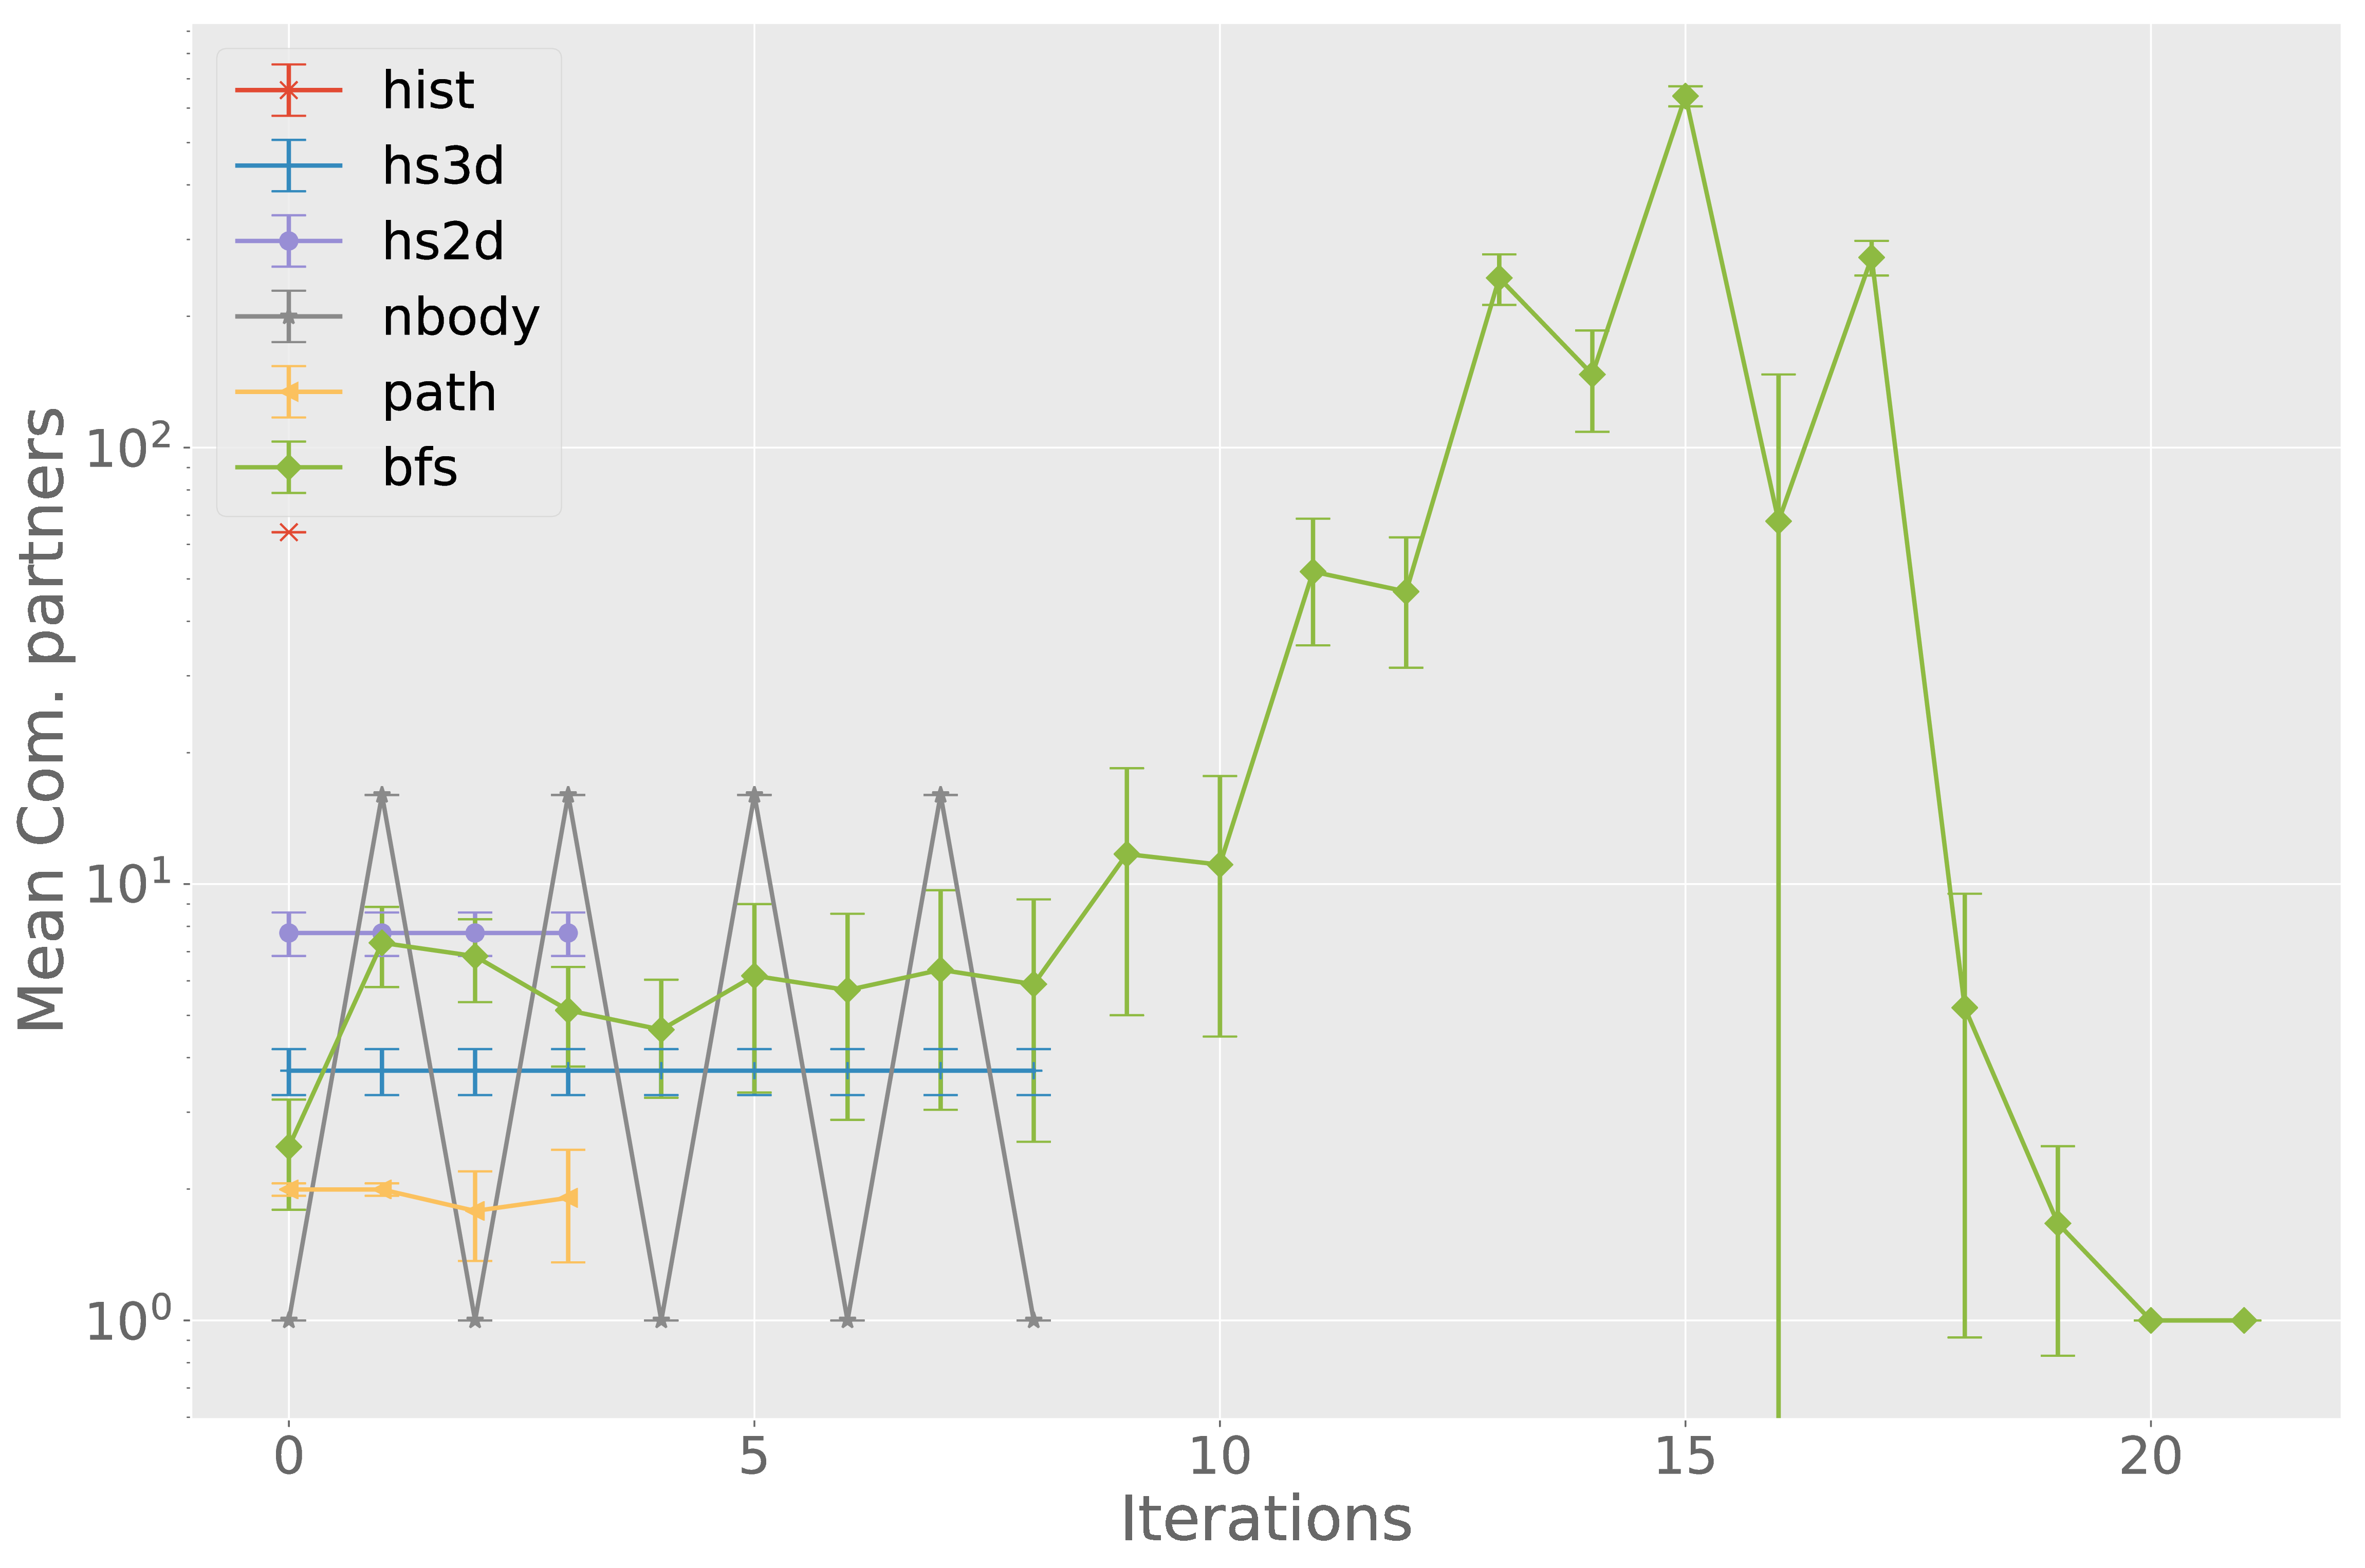
\includegraphics[width=\textwidth]{../../../Global-Memory-Tracing/memtrace-pass/plots/transmission-regularity}
	\caption{Mean out-degree of CTAs, per iteration}
	\label{philandering}
\end{figure}
	\chapter{Conclusion}
The first goal of this work was to use compilers to create  instrumentation, that makes detailed communication analysis in
GPU applications possible. GPUs are shared memory system and information can only be passed via global memory. Therefore, global memory operations are instrumented to create detailed memory access traces. The implemented solution introduces code on both, host and device to create a dynamic producer-consumer buffer system, allowing unlimited data generation. Host side modifications are performed in a Clang front-end plugin, as they are rather trivial.
Due to lowering and canonicalizations by the compiler, identifying global memory access instructions in device code is not straight forward and requires detailed code analysis and transformation. Analysis and transformation happen in 
LLVM IR, which allows a more efficient code analysis due to it's SSA properties.

Using the memory traces created by the instrumented, chapter \ref{eval} analysed the communication, as defined in \ref{methodik}. All applications showed that at least 30\% of all writes is later consumed by a communication partner. Both, incoming and outgoing communication has collective tendencies is and is rarely point-to-point. Communication is dominated by few different messages sizes in each application, usually packed tightly in memory. How the number
of communication partners and the communicated volumes behave over time, depends on the type of applications. Regular application with one kernel show no variance. Regular applications with multiple kernels show fluctuations, depending on the
kernel. Irregular applications show growing irregularities over time. Analysing the bisection volume shows, that most applications would benefit from more efficient GPU-to-GPU communication, as the share of data communicated across 
a bisection can be substantial. Only one application showed communication that could span several supersteps.

\section{Future Work}
The work on this project can be continued on both the tooling and the analysis aspect. For the tooling, a more complex trace
format that allows compressing coalesced memory access and the expression of access ranges of warp can reduce the impact on 
the runtime. Adding additional analysis features, like \verb|inline asm| for ptx analysis and the support for macros 
line \verb|ldg()| increase the range of applications that can be traced. To increase the range of supported applications, support of OpenCL could be implemented.

The analysis can be extended in both breadth and depth. Analysing more application can yield new insights, not yet present
in the analysis. A deeper analysis of specific applications can lead to an improved understanding of a single application,
revealing options for optimization.

Ultimately, a model for multi-gpu scalability could be derived from the analysis data.

\bibliographystyle{ieeetr}
\bibliography{report}
\begin{appendices}
	\pagenumbering{Roman}
	\setcounter{page}{4}
\chapter{Instrumentation}
Instrumenting an application at compile time happens in two steps. The first step is the instrumenting all 
source file containing:
\begin{itemize}
	\item Kernel Calls
	\item Kernel and \verb|__device__| function definitions
	\item Kernel \verb|__device__| functoin declarations
\end{itemize}

Each file needs to be parsed separately. For each file, a new file with the prefix 'augmented-' is created. This is then used for
the further build process. Compile units bear some problems with kernels defined and declared in \verb|.cu| files, which are then included
in other files. The easiest workaround is to copy the kernel into the file including it, and then only use the including file for instrumentation and build.

The following snipped is an example how to augment a kernel file.
\begin{lstlisting}[style=C]
clang++ -Xclang -load -Xclang "clang-plugin/libMemtrace-AA.so"
	 -Xclang -plugin -Xclang cuda-aug -Xclang -plugin-arg-cuda-aug 
	 -Xclang -f -Xclang -plugin-arg-cuda-aug -Xclang ./augmented-kernel.cu 
	 -I$CUDASYS/samples/common/inc -I. -I../utils
     --cuda-path=$CUDASYS -std=c++11 -E application/kernel.cu 
\end{lstlisting}

Next, the host and device utils are compiled, for later linking with the application.
\begin{lstlisting}[style=C]
// Host
clang++ -c -L$CUDASYS/lib64 --cuda-path=$CUDASYS 
 -I$CUDASYS/samples/common/inc -O1 --cuda-gpu-arch=sm_30
  -I$CUDASYS/include  -o hutils.o --std=c++11 -I. -I../utils
 ../utils/TraceUtils.cpp
// Device
clang++ -c -L$CUDASYS/lib64 --cuda-path=$CUDASYS 
 -I$CUDASYS/samples/common/inc -O1 --cuda-gpu-arch=sm_30
 -I$CUDASYS/include -o dutils.o --std=c++11 -I. -I../utils
 ../utils/DeviceUtils.cu
\end{lstlisting}
Next, all the augmented kernel files are compiled at once.
\begin{lstlisting}[style=C]
clang++ -c -Xclang -load -Xclang $LLVMPLUGIN  --cuda-path=$CUDASYS
 -I$CUDASYS/samples/common/inc --cuda-gpu-arch=sm_30 -L$CUDASYS/lib64  -O1
 -lcudart_static -m64  --std=c++11 -I. -I../utils -I<app-includes>
  ./augmented-kernel.cu ./augmented-kernel2.cu
\end{lstlisting}
Finally, all compiled files are linked together.
\begin{lstlisting}[style=C]
clang++ --cuda-path=$CUDASYS -I$CUDASYS/samples/common/inc --cuda-gpu-arch=sm_30 -L$CUDASYS/lib64  -O1
 -lcudart -ldl -lrt -L. -m64 --std=c++11 -I. -I../utils -I<app-includes>
 -o application dutils.o hutils.o augmented-kernel.o augmented-kernel2.o
\end{lstlisting}

During the execution one or more files are generated in the \verb|/tmp| folder. The files are named \verb|MemTrace-pipe-<n>|, one for
each stream.

\chapter{Post Processing}
Any software related to what that happens after the analysis, is stored in 'memtrace-pass/post-processing'.
The trace files can be parsed with the 'extract-subset.py' python3 script. From the original full trace, the communication 
subset is extracted. Three data structures are generated by 'extract-subset.py'. All structures are stored using pickle.
The data structures are of type 'AutoDict()', which is defined in 'TraceInc.py'
\begin{enumerate}
	\item Load/Store volumes, both total and during communication, for Kernels, CTAs and SMs. Separated by kernel and superstep.
	\begin{lstlisting}[style=C]
"KCV" : { // Kernel Communication Volume
	<kernel>: {
		<superstep>: {
			"Load" : <int>
			"Store": <int>
		}
	}
}
"KDV" : { // Total Kernel Data Volume
	<kernel>: {
		<superstep>: {
			"Load" : <int>
			"Store": <int>
		}
	}
}
"CCV" : { // CTA Communication Volume
	<kernel>: {
		<superstep>: {
			<CTA> : {
				"Load" : <int>
				"Store": <int>
			}
		}
	}
}

"CDV" : { // Total CTA Data Volume
	<kernel>: {
		<superstep>: {
			<CTA> : {
				"Load" : <int>
				"Store": <int>
			}
		}
	}
}
"SCV" : { // SM Communication Volume
	<kernel>: {
		<superstep>: {
			<SM> : {
				"Load" : <int>
				"Store": <int>
			}
		}
	}
}

"SDV" : { // Total SM Data Volume
	<kernel>: {
		<superstep>: {
			<SM> : {
				"Load" : <int>
				"Store": <int>
			}
		}
	}
}

	\end{lstlisting}
	\item Map of transfers, ordered by kernel, CTA and superstep.
	\begin{lstlisting}[style=C]
<source-kernels> : {
	<source-cta> : {
		<source-superstep> : {
			<recv-kernel>: {
				<recv-cta>: {
					<recv-superstep>: {
						'Size' : <int>
						'cnt'  : <int>
					}
				}
			}
		}
	}
}
	\end{lstlisting}
	\item All addresses involved in communication, with all operations performed on this address, in superstep order.
	\begin{lstlisting}[style=C]
{
	<address> : [
		{ // record
			"kernel": <kernel>
			"it"    : <superstep>
			"cta"	: <CTA-ID, xyz order>
			"addr"  : <address>
			"smid"  : <SM id>
			"size"  : <operation size in bytes>
			"type"  : <type of MOp>
		}
	]
}
	\end{lstlisting}
\end{enumerate}
\end{appendices}
\end{document}
